% !TeX root = skript.tex
Ein Zufallsgraph ist ein Modell einer Graphfamilie --- etwa wie eine Zufallsvariable ein Modell einer Zufallsgröße ist.
Der Zufallsgraph beschreibt also ein Ensemble von Graphen, das so entworfen sein kann, dass bestimmte Eigenschaften in den betrachteten Graphen verstärkt auftreten.
So maßgeschneiderte Zufallsgraphen werden oft als \emph{Netzwerkmodell} bezeichnet.

Das Forschungsfeld der Zufallsgraphen nahm mit den Arbeiten von Gilbert~\cite{gilbert_1959}, sowie Erd\H{o}s und R\'enyi~\cite{erdos_renyi_1960} Anfang der 1960er Jahre an Fahrt auf.
Die beiden Arbeiten definieren Zufallsgraphen, die zunächst für abstrakte Untersuchungen (z.B. die Probabilistische Methode) verwendet wurden.
Der Fokus auf die Modellierung von beobachteten Netzwerken kam erst später hinzu.
Dennoch spielen die Modelle in der Netzwerkforschung bis heute eine wichtige Rolle.
Wir werden sie daher bald genauer betrachten, fangen jedoch mit einem noch einfacheren Modell an.

\section{Der Zufallsgraph $\Gn$}
Ein Zufallsgraph $(\mathbb G, f)$ ist eine Wahrscheinlichkeitsverteilung $f\colon \mathbb G \to [0, 1]$ über einer Menge von Graphen $\mathbb G$.
Oftmals wird der Grundraum $\mathbb G$ durch eine Parametrisierung eingeschränkt; auch $f$ kann parametrisiert sein.

Das \aside{$\Gn$ Graphen} einfachste Modell ist $\Gn$, welches die Gleichverteilung über alle Graphen mit $n$ Knoten beschreibt.
Hierbei ist zu beachten, dass wir mit \emph{alle Graphen} in der Regel entweder alle \emph{gerichteten} oder alle \emph{ungerichteten} Graphen meinen.
Die Details der Analysen in den folgenden Kapiteln hängen von dieser Entscheidung ab --- allerdings ergeben sich meist keine qualitativen Unterschiede.
Daher werden wir oft den für uns einfacheren Fall wählen.
Je nach Wahl, ist der Grundraum von $\Gn$
\begin{align}
    \mathbb G_\text{ger}(n)  & =
    \twoset{G(V,E)}{|V| = n \land E \subseteq V \times V} \\\label{eq:gerichtet_gn}
    \mathbb G_\text{unge}(n) & =
    \twoset{G(V,E)}{|V| = n \land  E \subseteq \twoset{\set{u,v}}{u,v \in V \text{ mit } u \ne v}}.
\end{align}

\noindent Die Wahrscheinlichkeitsverteilung $f$ folgt dann als $f_{\gGn}(G) = 1 / | \gGn |$, oder konkret:
\begin{align}
    f_{\mathbb G_\text{ger}(n)}(G)  & =  \frac{1}{| \mathbb G_\text{ger}(n) |} = 2^{-n^2}\label{eq:gleichverteilt_gerichtet_gn} \\
    f_{\mathbb G_\text{unge}(n)}(G) & =  \frac{1}{| \mathbb G_\text{unge}(n) |} = 2^{-\binom n 2} = 2^{-\frac{n(n-1)}{2}}.
\end{align}

Die geschlossene Form $| \mathbb G_\text{ger}(n) | = 2^{n^2}$ in \cref{eq:gleichverteilt_gerichtet_gn} ergibt sich daraus, dass ein gerichteter Graph $n^2$ potentielle Kanten hat (die Adjazenzmatrix hat $n \times n$ Einträge).
Für jede dieser Kanten haben wir unabhängig genau zwei Möglichkeiten: sie existiert oder eben nicht.
Analog sieht es für die $\binom n 2$ möglichen Kanten in einem ungerichteten Graphen aus.

Beachte aber auch, dass formal \cref{eq:gerichtet_gn} und \cref{eq:gleichverteilt_gerichtet_gn} widersprüchlich scheinen.
In \cref{eq:gerichtet_gn} fordern wir nur, dass die Knotenmenge~$V$ die Kardinalität $|V| = n$ hat.
Offensichtlich gibt es unbeschränkt viele dieser Wahlen; für $n=3$ z.B. $\set{1,2,3}$, $\set{2,3,4}$, \ldots, $\set{k, k+1, k+2}$ für alle $k \in \mathbb N$.
Die Wahl der Knotenbezeichner hat jedoch keinen Einfluss auf die Netzwerkeigenschaften.
Daher werden wir in dieser Veranstaltung grundsätzlich annehmen, dass die Knotenmengen in irgendeiner Form fixiert sind, z.B. als $V = \set{1, \ldots, n} = [n]$ oder $V = \set{v_1, \ldots, v_n}$.

\bigskip

Ist das $\Gn$ Modell aber nun realistisch?
Das hängt davon ab, was wir mit ihm bezwecken und was wir mit \emph{realistisch} meinen.
Es ist aber sicherlich nicht geeignet, um gängige Netzwerke zu beschreiben.
Dies liegt unter anderem daran, dass $\Gn$ oft Graphen mit vielen Kanten erzeugt;
intuitiv hat \glqq jeder zweite Graph\grqq{} mindestens die Hälfte aller möglichen Kanten.

\begin{figure}[t]
    \begin{center}
        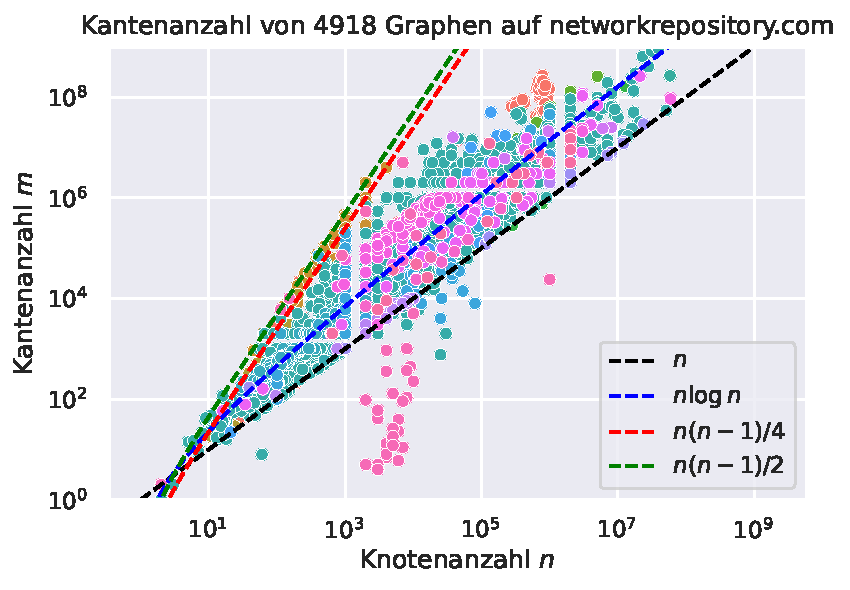
\includegraphics[width=0.5\textwidth]{data/network-rep-edges.pdf}%
        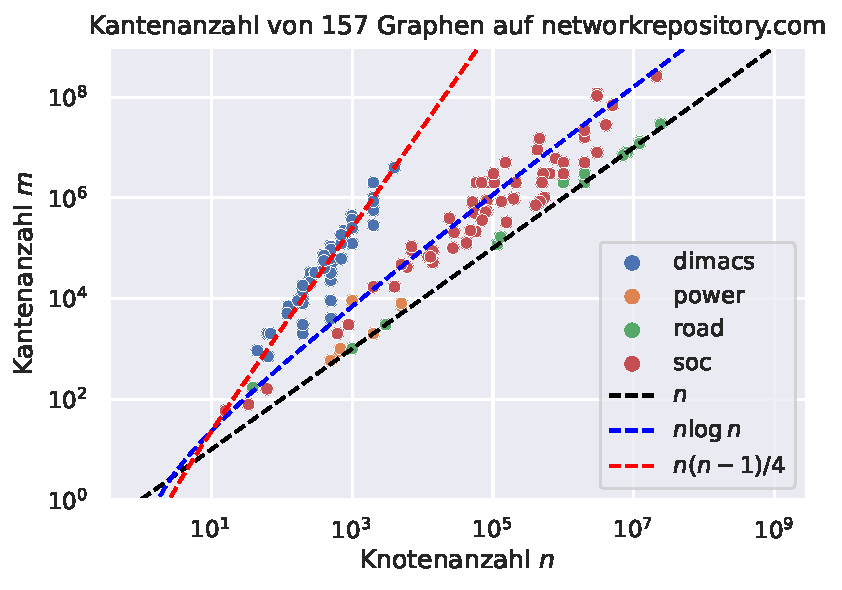
\includegraphics[width=0.5\textwidth]{data/network-rep-edges-thin.pdf}%
    \end{center}
    \caption{
        Die Verteilung der Kantenanzahl in verschiedenen Netzwerken auf~\cite{networkrepository}.
        Die Farben der einzelnen Punkte geben an, aus welchem Bereich die Netzwerke stammen.
    }
    \label{fig:kantenanzahl}
\end{figure}


\begin{observation}
    Sei $G(V,E)$ ein Graph, der zufällig aus $\Gn$ mit $n > 1$ gezogen wurde.
    Dann gilt für gerichtete Graphen $\prob{|E| \ge n^2 / 2} \ge 1/2$ und für ungerichtete Graphen $\prob{|E| \ge \binom{n}{2} / 2} \ge 1/2$.
\end{observation}

\begin{proof}
    Im Folgenden betrachten wir nur gerichtete Graphen; der Beweis läuft analog für ungerichtete Graphen.
    Stellen wir uns einen beliebigen Graphen~$G(V, E)$ vor.
    Dann sei $\bar G(V, \bar E)$ sein Komplement, d.h. für alle möglichen Kanten gilt:
    \begin{equation}
        \forall e \in V\times V\colon \quad\quad e \in \bar E \Leftrightarrow e \notin E
    \end{equation}
    Beobachte, dass es eine Bijektion zwischen allen Graphen in $\mathbb G$ und ihren Komplementen gibt: jeder Graph hat ein eineindeutiges Komplement.
    Per Konstruktion gilt außerdem:
    \begin{eqnarray}
        E \cup \bar E &=& V \times V\\
        \Rightarrow |E| + |\bar E| &\ge& n^2\\
        \Rightarrow \max(|E|, |\bar E|) &\ge& n^2 / 2.
    \end{eqnarray}

    Für jeden Graph~$G$ gilt also, dass entweder $G$ selbst oder sein Komplement~$\bar G$ mindestens $n^2 / 2$ Kanten hat.
    Da wir $G$ und $\bar G$ je mit gleicher Wahrscheinlichkeit ziehen, gilt $\prob{|E| \ge n^2 / 2} \ge 1/2$.
\end{proof}

\section{Kantenanzahl in beobachteten Netzwerken}\label{sec:kanten-in-beobachteten-netzen}
Wie viele Kanten haben echte Netzwerke? Hierzu führen wir ein Experiment durch:
wir nutzen die Datenbank \url{https://networkrepository.com/}, die über 5000 Netzwerke aus unterschiedlichen Bereichen enthält~\cite{networkrepository}.
In \cref{fig:kantenanzahl} zeichnen wir die Kantenanzahl als Funktion der Knotenanzahl.
Zwei Eigenschaften fallen direkt auf:
\begin{enumerate}
    \item Die Kantendichte hängt vom Netzwerktyp ab.
    \item Es sind fast immer deutlich weniger als die Hälfte der Kanten vorhanden.
\end{enumerate}

\subsection{Netzwerktypen haben unterschiedliche Kantendichten}
Betrachten wir die erste Beobachtung genauer, indem wir Straßennetze und Freundschaftsnetze vergleichen.
Wir modellieren ein Straßennetz dadurch, dass Adressen (Häuser, Kreuzung, usw.) als Knoten und Straßen als Kanten dargestellt werden.
Diese Netze \aside{Straßennetze} sind im wesentlichen ein zwei-dimensionales Konstrukt.
Wenn wir Tunnel, Brücken und der gleichen ignorieren, verlaufen Straßen nicht über einander.
Daher erwarten wir, dass die Graphen von Straßennetzen fast planar sind.
Nach dem Eulerischen Polyedersatz erfüllen einfache, \aside{planare Graphen} planare und zusammenhängende Graphen:
\begin{equation}
    |E| \le 3 |V| - 6
\end{equation}
Knoten in einem Straßennetz sollten also im Schnitt höchstens 6 Nachbarn haben.

In \aside{Freundschaftsnetze} sozialen Netzwerken ist die Situation anders ---
stellen wir uns etwa einen Freundschaftsgraphen vor, in dem Knoten die Nutzer eines sozialen Netzwerks sind und Kanten eine Freundschaft anzeigen.
Im Jahr 2014, hatten Facebook-Nutzer im Schnitt mehr als 300 Freunde (mehr dazu später).
Dies ist offensichtlich deutlich mehr als in planaren Graphen möglich wäre.
Ganz ähnlich sieht es mit anderen sozialen Netzen aus: ein durchschnittlicher Erwachsener kennt deutlich mehr als 6 andere Menschen persönlich (oft werden Zahlen zwischen 100 und 300 genannt).

\subsection{Die meisten Netzwerke sind dünn}
In \cref{fig:kantenanzahl} hat nur ein verschwindend geringer Anteil der Netzwerke mindestens die Hälfte aller Kanten (d.h. ist oberhalb der roten Linie).
Wie erklärt sich das?
In der Regel verursacht eine Kante Kosten:
eine Straße muss gebaut werden, eine Freundschaft muss aufrecht erhalten werden (Zeitinvestment), eine Nachricht muss geschrieben werden, etc.
Daher gibt es in den meisten Netzwerken einen gewissen Selektionsdruck, der dazu führt, dass jeder Knoten nur ausgewählte Nachbarn besitzt.
Wir klassifizieren Netzwerktypen, die auffallend viele oder wenig Kanten haben:

\begin{definition}
    Graphen \aside{dünne und dichte Graphen} mit $n$ Knoten und $m$ Kanten heißen \emph{dünn} (engl. sparse), wenn $m = \Oh{n \log n}$ gilt, und \emph{dicht} wenn $m = \Omega(n^2)$.
\end{definition}

\begin{remark}
    Aufgrund der asymptotischen Definition verwendet man \emph{dünn} und \emph{dicht} eher für Graphfamilien (so auch Zufallsgraphen) als für einzelne Instanzen.
    Manche abweichende Definitionen fordern für \emph{dünne} Graphen $m = \Oh{n}$.
    Wir nutzen hier $\Oh{n\log n}$, um soziale Netzwerke mit einzubeziehen.
\end{remark}

\section{Die Zufallsgraphen $\Gnm$ und $\Gnp$}
Das $\Gn$ Modell verfügt über keinen Mechanismus um Kanten auszudünnen.
Wir benötigen also Prozesse, die weniger dichte Graphen erzeugen können ---
am besten parametrisiert, damit wir unterschiedlichen Netzwerktypen Rechnung tragen können.
Im Folgenden betrachten wir zwei solcher Modelle.

Das \Gnm-Modell \aside{Erd\H{o}s-R\'enyi Graphen \Gnm} von P.~Erd\H{o}s und A.~R\'enyi beschreibt die Gleichverteilung über allgemeinen Graphen mit $n$ Knoten und $m$ Kanten, d.h. wir betrachten die Grundmenge
\begin{equation}
    \gGnm = \twoset{G}{G=(V,E) \in \mathbb G(n) \text{ und } |E| = m}.
\end{equation}
Da gleichverteilt gewählt wird, gilt für die Wahrscheinlichkeitsverteilung~{$f\colon \mathbb G \to [0,1]$}
\begin{equation}
    f(G) = \frac{1}{| \gGnm |} \quad \text{ für alle } G \in \gGnm.
\end{equation}

\begin{exercise}
    Berechne $|\gGnm|$ für gerichtete und ungerichtete Graphen.
\end{exercise}

E.~Gilbert \aside{Gilbert-Graphen \Gnp} beschreibt ein ähnliches Modell, das \Gnp-Modell --- das oft fälschlicherweise \glqq Erd\H{o}s-R\'enyi-Modell \grqq{} genannt wird.
Um das Modell zu beschreiben, weichen wir von der bisherigen expliziten Definition der Grundmenge und Verteilung ab.
Stattdessen, spezifizieren wir eine randomisierte Konstruktionsvorschrift:
\begin{enumerate}
    \item Erzeuge $n$ Knoten $V = \{v_1, \ldots, v_n\}$.
    \item Setze $E = \emptyset$.
    \item Für jedes Paar von Knoten $(v_i, v_j)$ führe ein unabhängiges Bernoulli Experiment durch.
          Mit Wahrscheinlichkeit $p$ füge $(v_i, v_j)$ als Kante zu $E$ hinzu.
    \item Gebe den Graphen $G=(V, E)$ zurück.
\end{enumerate}

\noindent
Graphisch kann man sich also \Gnp als Adjazenzmatrix vorstellen, in der die Einträge unabhängig voneinander mit Wahrscheinlichkeit $p$ auf $1$ gesetzt werden:

\begin{center}
    \begin{tikzpicture}
        \node (mat) at (0,0) {
            $\begin{pmatrix}
                    1 & 0 & 1 & 0 & 0 \\
                    0 & 1 & 1 & 0 & 1 \\
                    0 & 1 & 0 & 1 & 0 \\
                    1 & 0 & 1 & 0 & 0 \\
                    1 & 0 & 0 & 0 & 1 \\
                \end{pmatrix}$
        };

        \node[anchor=west, align=left, xshift=4em] (label) at (mat.east) {
            $\begin{cases}1 & \text{mit Wahrscheinlichkeit } $p$ \\
                    0 & \text{mit Wahrscheinlichkeit } 1-p
                \end{cases}$
        };

        \path[draw, thick, bend right, ->] (label.west) to (mat.center);
    \end{tikzpicture}

\end{center}

\begin{exercise}
    Die genannte Konstruktion erzeugt gerichtete Graphen.
    Zeige, wie die Konstruktion so angepasst werden kann, dass gerichtete Graphen ohne Eigenschleifen erzeugt werden.
    Wie verändert sich dann die Adjazenzmatrix?
    Wie verhält es sich mit ungerichteten Graphen?
\end{exercise}

Durch ihre einfache Konstruktion sind beide Zufallsgraphen bis heute sehr verbreitete Modelle in der Netzwerkforschung.
Wir werden jedoch sehen, dass viele Eigenschaften von echten Netzwerken auch von \Gnp oder \Gnm-Graphen nicht beschrieben werden können.

\subsection{Anzahl von Kanten in \Gnp}\label{subsec:anzahl_kanten_in_gnp}
Während bei \Gnm Graphen die Anzahl der Kanten durch den Parameter~$m$ fixiert ist, ist $|E|$ bei \Gnp Graphen eine Zufallsvariable.

\begin{lemma}\label{lemma:erwartete_kanten_in_gnp}
    Die \aside{Erwartete Kantenanzahl $\expv{|E|}$ in \Gnp} erwartete Kantenanzahl~$m$ in einem gerichteten \Gnp Graphen ist \begin{equation*} \expv{m} = p n^2. \qedhere \end{equation*}
\end{lemma}

\begin{proof}
    Fixiere einen Graphen~$G=(V,E)$ aus \Gnp.
    Für jede Kante $(u,v)$ definiere die Indikatorvariable $I_{u,v}$, die anzeigt, ob die Kante $(u,v) \in E$ enthalten ist:
    \begin{equation}
        I_{u,v} = \begin{cases}
            1 & \text{ falls } (u,v) \in E \\
            0 & \text{ sonst }
        \end{cases}
    \end{equation}

    \noindent Somit folgt Anzahl der Kanten~$m$ in $G$ als Summe über die Indikatorvariablen
    \begin{equation}
        |E| = \sum_{u,v \in V} I_{u,v} = \left(\sum_{(u,v) \not\in E} 0 \right) +  \left(\sum_{(u,v) \in E} 1\right).
    \end{equation}

    \noindent Per Definition von \Gnp gilt $\prob{I_{u,v} {=} 1} = p$ und $\prob{I_{u,v} {=} 0} = 1-p$.
    Somit folgt für den Erwartungswert jeder Indikatorvariable
    \begin{equation}
        \expv{I_{u,v}} = 1 \cdot p + 0 \cdot (1-p) = p \quad \text{unabhängig für alle } u, v \in V.
    \end{equation}

    \noindent Durch die Linearität des Erwartungswertes folgt schließlich
    \begin{equation}
        \expv{|E|} = \sum_{u,v \in V} \expv{I_{u,v}} = \sum_{u,v \in V} p = p n^2. \qedhere
    \end{equation}
\end{proof}

\begin{exercise}
    Zeige, dass die erwartete Anzahl an Kanten in einem ungerichteten \Gnp Graphen $\expv{|E|} = \binom{n}{2} p = p n(n-1)/2$ beträgt.
\end{exercise}

\begin{exercise}
    Zeige, dass $\Gn = \mathcal G(n, 1/2)$.
\end{exercise}

\bigskip

Wie wir am Beweis von \cref{lemma:erwartete_kanten_in_gnp} sehen, ergibt sich die Kantenanzahl~$m$ als Summe von unabhängigen Bernoulli Zufallsvariablen;
sie ist also selbst eine Zufallsvariable und binomial verteilt.
Da uns die Binomialverteilung regelmäßig begegnen wird, wollen wir uns diese kurz in Erinnerung rufen.
\begin{definition}
    Die \aside{Binomialverteilung.} Binomialverteilung $B_{N, p}(k)$ beschreibt die Wahrscheinlichkeit, dass bei $N$~unabhängigen Bernoulli Experimenten mit Wahrscheinlichkeit $p$ genau $k$ Experimente erfolgreich sind.
    Es gilt \aside{\ \\ \ \\ \ \\ Binomialkoeffizient $\binom{n}{k} = \frac{n!}{(n-k)!k!}$}
    \begin{eqnarray*}
        \prob{B_{N,p} {=} k} &=& \binom{N}{k} p^k (1-p)^{N-k} \\
        \expv{B_{N,p}} &=& Np \\
        \varv{B_{N,p}} &=& Np(1-p),
    \end{eqnarray*}
    wobei $\expv{B_{N,p}}$ und $\varv{B_{N,p}}$ den Erwartungswert und die Varianz der Binomialverteilung beschreiben.
\end{definition}

Die Standardabweichung $\sigma = \sqrt{\varv{B_{N,p}}} \le \sqrt{\expv{B_{N,p}}}$ ist also relativ klein.
Wir können daher davon ausgehen, dass für hinreichend großes $N$ die Binomialverteilung recht stark um ihren Erwartungswert $Np$ konzentriert ist.
Daher sagen wir, dass \Gnm und \Gnp mit $p=m/n^2$ asymptotisch (d.h. für $n \to \infty$) äquivalent sind.
Häufig ist es jedoch einfacher \Gnp Graphen zu analysieren, da ---im Gegensatz zu \Gnm Graphen--- alle Kanten unabhängig gezogen werden.

\section{Effizientes Ziehen von \Gnp Graphen}
Zufallsgraphen sind nicht nur in der theoretischen Analysen von Prozessen und Algorithmen nützlich, sondern auch für empirische Untersuchungen.
Nehmen wir etwa an, dass wir einen Algorithmus implementiert haben und dessen Geschwindigkeit oder Qualität vermessen möchten.
Dann können Zufallsgraphen unter anderem aus folgenden Gründen nützlich sein:
\begin{itemize}
    \item Wenn die Generatorsoftware vorhanden ist, können wir synthetische Instanzen in quasi unbeschränkter Menge generieren.
    \item Parametrisierte Generatoren erlauben den Einfluss gewisser Eigenschaften detailliert zu analysieren; z.B. Skalierungsexperimente.
    \item Beobachtete Graphen haben oft \glqq Rauschen\grqq, d.h. nicht verstandene oder insignifikante Strukturen, die Messungen verfälschen können.
          Zufallsgraphen, hingegen, haben i.d.R. eine gut verstandene Struktur, die es uns oft ermöglicht vor dem Testen Hypothesen aufzustellen.
    \item Einige Generatoren können anhand eines fixierten Startzustands (Random-Seed) dieselben Graphen wiederholt erzeugen.
          Wir müssen also die Eingaben nicht speichern/transferieren und können dennoch reproduzierbare Experimente durchführen.
\end{itemize}

\noindent Da in verschiedenen wissenschaftlichen Communities der Begriff \glqq Generator\grqq{} unterschiedlich benutzt wird, hier noch eine Definition:
\begin{definition}
    Ein \aside{Graphgenerator} Graphgenerator ist ein Algorithmus, der einen Graphen aus einem Netzwerkmodell erzeugt.
    Dieser respektiert die Verteilung des zugrundeliegenden Modells.
\end{definition}

\subsection{Ein naiver Ansatz}
Betrachten wir folgenden Graphgenerator für \Gnp Graphen, der im wesentlichen eine 1:1 Implementierung der Definition von \Gnp ist:

\begin{algorithm}[H]
    \KwIn{Anzahl der Knoten~$n$ und Verbindungswahrscheinlichkeit~$p$}
    \KwOut{Adjazenzmatrix eines zufälligen Graphs $G \follows \Gnp$}
    Allokiere eine Matrix $A[1..n, 1..n]$\;
    \For{$1 \le i \le n$}{
        \For{$1 \le j \le n$}{
            Setze $A[i,j] \gets \begin{cases}
                    0 & \text{mit Wahrscheinlichkeit } 1-p \\
                    1 & \text{mit Wahrscheinlichkeit } p
                \end{cases}$\;
        }
    }
    Gebe $A$ zurück
    \caption{Naiver Graphgenerator für \Gnp Graphen}
    \label{alg:naive-gnp}
\end{algorithm}

Um \aside{Annahme: aus einfachen Verteilungen kann in kostanter Zeit gezogen werden.} die Laufzeit dieses Algorithmus bestimmen zu können, treffen wir in dieser Veranstaltung folgende Annahme.
Wir können unter anderem aus folgenden Zufallsverteilungen in konstanter Zeit ziehen:
\begin{itemize}
    \item Ganzzahlig uniform aus $[a, b]$ für $a, b \in \mathbb{Z}$.
    \item Gleitkommazahl uniform aus $[a, b]$ für $a, b \in \mathbb{R}$.
    \item Bernoulli (folgt aus vorherigem Punkt)
    \item Binomial, Geometrisch (siehe \cref{{sec:inversionsmethode}}), Hypergeometrisch, Poisson
\end{itemize}

Tatsächlich können die meisten dieser Verteilungen nur in \emph{erwartet} konstanter Zeit gezogen werden, praktisch sind die Fluktuationen jedoch so klein, dass wir sie vernachlässigen können.
Das erlaubt es uns auf die Eigenschaften der Graphgeneratoren zu konzentrieren.

\begin{lemma}
    \label{lem:naive-gnp}
    Der Algorithmus \ref{alg:naive-gnp} erzeugt einen \Gnp Graphen in $\Theta(n^2)$ Zeit.
\end{lemma}

\begin{exercise}
    Beweise das Lemma.
\end{exercise}

Nun könnte man argumentieren, dass dieser naive Algorithmus bereits optimal ist:
Die Ausgabe hat Größe $\Theta(n^2)$ und somit wir benötigen $\Omega(n^2)$ Zeit, um die Ausgabe zu erzeugen.
Außerdem hat ein Graph mit $p=\Omega(1)$ erwartete $\Theta(n^2)$ Kanten, was wiederum die Laufzeit von unten beschränkt.

Diese Worst-Case Schranken passen jedoch nicht zu unserer Beobachtung in \cref{sec:kanten-in-beobachteten-netzen}, dass Graphen in der freien Wildbahn meist dünn sind.
Es wäre schön, wenn wir diese Graphen schneller erzeugen könnten, jedoch ist \cref{alg:naive-gnp} für alle $p$ gleich \glqq schnell\grqq.
Hier \aside{ausgabesensitive Algorithmen} helfen \emph{ausgabesensitive Algorithmen} (output-sensitive algorithm), deren Laufzeit maßgeblich durch die Größe der Ausgabe bestimmt wird;
die meisten Generatoren, die wir betrachten werden, fallen genau in diese Kategorie.

Ausgabesensitive \aside{Kantenlisten} Algorithmen müssen jedoch eine Ausgabedatenstruktur nutzen, die sich an die Größe anpasst.
Eine Matrix hat immer dieselbe Größe unabhängig davon, wie viele Einsen (Kanten) vorhanden sind.
Wir werden im Folgenden fast immer eine Kantenliste annehmen, die nur $\Oh{1}$ Speicherworte pro Kante benötigt.

\subsection{Ziehen mit zufälligen Sprüngen}\label{subsec:gnp_zufaellige_spruenge}
Wie können wir nun \cref{alg:naive-gnp} verändern, so dass er ---analog zu Kantenlisten--- keine Arbeit für Nichtkanten verrichtet?
Idee: Wir müssen diese einfach überspringen!
Aber woher wissen wir wo \glqq Nullen\grqq{} gezogen werden, bzw. wie viele Nullen müssen wir überspringen?
Zählen können wir sie nicht ohne wieder direkt quadratische Arbeit zu verrichten.

Ganz \aside{Effizientes Ziehen durch Überspringen von Nullen} einfach: wir fragen uns wie viele Nullen~$\ell$ \cref{alg:naive-gnp} gesetzt hätte und überspringen diese.
Zwischen diese zufälligen Sprünge setzen wir dann die Einsen ein.
Wenn wir nun $\ell$ aus einer geeigneten Verteilung ziehen, haben wir zwei unterschiedliche Zufallsprozesse, deren Ausgabe aber nicht unterscheidbar ist.
Generalisierungen dieser Methode werden uns noch häufiger begegnen.

Zur \aside{Statt $n \times n$ Matrix, nehmen wir einen $n^2$ Vektor an} Vereinfachung stellen wir uns die Adjazenzmatrix~$A = (a_{ij})_{ij}$ als einen Vektor~$B = (b_k)_k$ vor, der dadurch entsteht, dass wir die Zeilen hinter einander anfügen (row-major layout).
Eintrag $a_{ij}$ wird also mit $b_{(i-1)n + j}$ identifiziert.
Dann besteht unsere Aufgabe darin genau alle $b_k$ zu finden, die den Wert $1$ haben.

\begin{equation}
    \Big(\quad \cdots \overbrace{1}^{b_k} \ \underbrace{0 \ \ 0\ \ 0 \ \cdots\ \ 0\ \ 0\ \ 0}_{\text{$\ell$ zusammenhängende Nullen}}\  \overbrace{1}^{b_{k + 1+ \ell}} \cdots \quad \Big)
\end{equation}

\noindent
Sei $X$ die \aside{Anzahl Nullen $X$ ist geometrisch verteilt} Zufallsvariable, welche die Anzahl der Nullen nach einer Eins modelliert.
\begin{eqnarray}
    \prob{X = 0} &=& \prob{\text{Nächster Versuch: 1}} = p \\
    \prob{X = 1} &=& \prob{\text{Nächster Versuch: 0, dann 1}} = (1 - p)p \\
    \prob{X = 2} &=& \prob{\text{Nächster Versuch: 0, dann 0, dann 1}} = (1 - p)^2 p \\
    &\vdots& \\
    \prob{X = \ell} &=& (1 - p)^\ell p
\end{eqnarray}

\noindent Die Zufallsvariable ist also \emph{geometrisch verteilt} mit Parameter $p$.
Es ergibt sich also der folgende einfache Algorithmus:

\begin{algorithm}[H]
    \KwIn{Anzahl der Knoten~$n$ und Verbindungswahrscheinlichkeit~$p$}
    \KwOut{Kantenliste $E$ eines zufälligen Graphs $G \follows \Gnp$}
    Initialisiere eine leere Kantenliste $E$\;
    $k \gets -1$\;
    \While{true}{
        $\ell \gets \text{ziehe die Sprungweite aus einer geometrischen Verteilung mit Parameter $p$}$\;
        $k \gets k + \ell + 1$\;

        \If{$k < n^2$}{
            $(i, j) \gets (\lfloor k / n \rfloor$, \ k \text{ mod } n)\;
            $E \gets E \cup \{(i+1, j+1)\}$\;
        } \Else {
            Gebe $E$ zurück und beende\;
        }
    }
    \caption{Generator für \Gnp Graphen mit zufällige Sprüngen}
    \label{alg:linear-gnp}
\end{algorithm}

\begin{lemma}
    \label{lem:linear-gnp}
    Algorithmus \ref{alg:linear-gnp} erzeugt Graph $G(V, E) \follows \Gnp$ in $\Theta(|E|)$ Zeit.
\end{lemma}

\begin{exercise}
    Beweise das Lemma.
\end{exercise}
\begin{exercise}
    Passe \cref{alg:linear-gnp} für ungerichtete Graphen an.
\end{exercise}

Jetzt müssen wir nur noch herausfinden, wie wir geometrische Sprünge effizient ziehen können.
Hierzu kommt meist die Inversionsmethode zum Einsatz.

\subsection{Inversionsmethode: Ziehen aus der geometrischen Verteilung}
\label{sec:inversionsmethode}

\begin{figure}[t]
    \begin{center}
        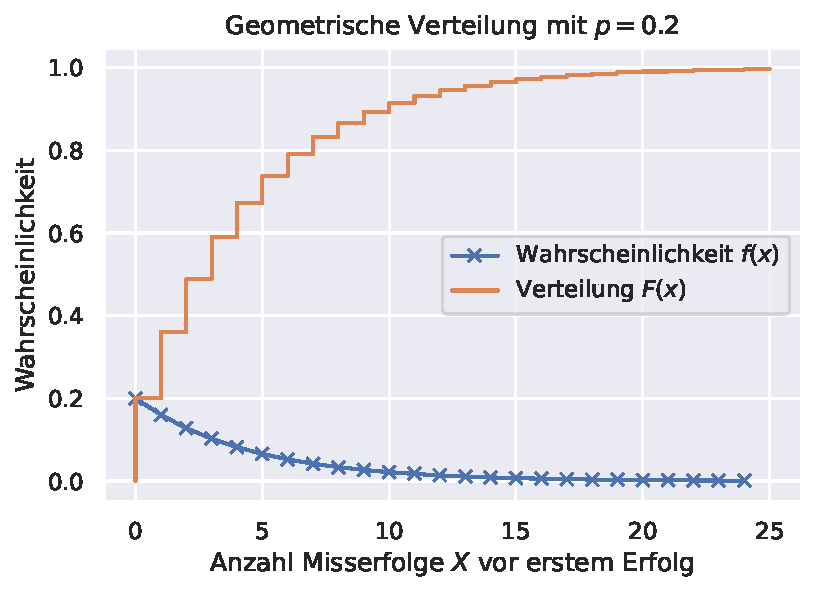
\includegraphics[width=0.5\textwidth]{data/geometric-distr.pdf}%
        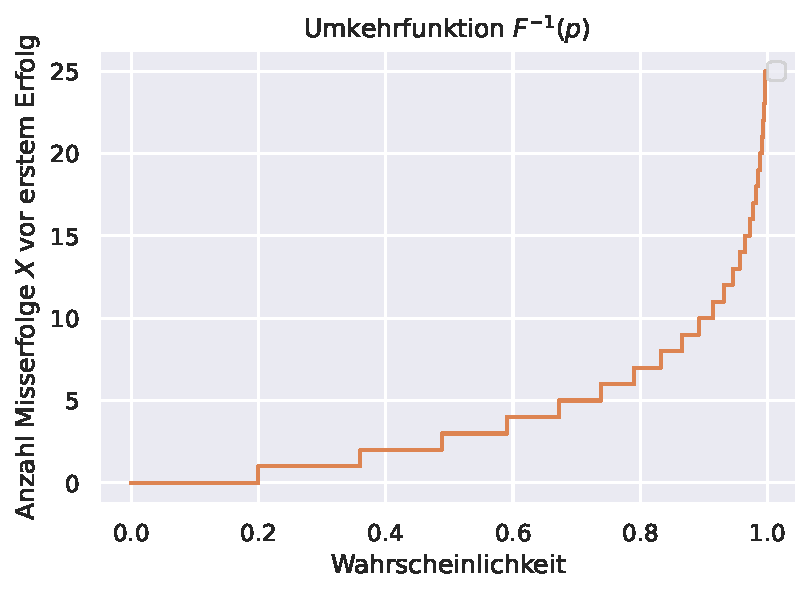
\includegraphics[width=0.5\textwidth]{data/geometric-distr-inv.pdf}
    \end{center}

    \caption{
        Wahrscheinlichkeitsverteilung und kumulative Verteilungsfunktion einer geometrischen Verteilung mit Parameter $p = 0.2$ (links).
        Die rechte Abbildung zeigt die \glqq Umkehrfunktion\grqq{} $F^{-1}(p)$ der kumulativen Verteilungsfunktion $F(x)$.
    }
    \label{fig:geometric-distr}
\end{figure}

Die \aside{Inversionsmethode: effizientes Ziehen falls Umkehrfunktion bekannt} Inversionsmethode (inversion transform method) ist ein allgemeines Verfahren, um eine uniforme Zufallsvariable in eine andere Verteilung zu übersetzen.
Wir betrachten die Methode hier am Beispiel der geometrischen Verteilung.
In \cref{fig:geometric-distr} ist die Wahrscheinlichkeitsverteilung $f(\ell)$ und die kumulative Verteilungsfunktion $F(\ell)$ einer geometrischen Verteilung mit Parameter $p = 0.2$ gezeigt.
%
%Da $f(\ell)$ ist eine Wahrscheinlichkeitsverteilung ist, muss $\sum_{\ell=0}^{\infty} f(\ell) = 1$ gelten.
Betrachten wir die konkreten ersten drei Werte der Funktionen:

\begin{center}
    \begin{tabular}{l|p{0.2\textwidth}p{0.25\textwidth}p{0.35\textwidth}}
                  & $\ell = 0$ & $\ell = 1$              & $\ell = 2$                              \\\hline\hline
        $f(\ell)$ & $p =0.2$   & $(1 {-} p)p = 0.16$     & $(1 {-} p)^2p = 0.128$                  \\
        $F(\ell)$ & $p =0.2$   & $p{+}(1 {-} p)p = 0.36$ & $p{+}(1 {-} p)p{+}(1 {-} p)^2p = 0.488$
    \end{tabular}
\end{center}
\vspace{1em}

Ein Generator sollte also z.B. den Wert $0$ mit Wahrscheinlichkeit 20\,\% ausgeben.
Da wir einen deterministischen Algorithmus konstruieren möchten, brauchen wir eine Quelle für den Zufall:
wir erwarten eine uniforme Zufallsvariable $U \in [0, 1)$ als Eingabe.
Wir können also z.B. prüfen:
\begin{itemize}
    \item Wenn $U < 0.2$ ist, dann gebe den Wert $0$ zurück.
          Da $U$ uniform verteilt ist, ist die Wahrscheinlichkeit für $U < 0.2$ genau $0.2$.

    \item Falls nicht prüfen wir, ob $U < 0.36 = f(0) + f(1) = F(1)$ ist. Falls ja, geben wir den Wert $1$ zurück.
          Da $U$ uniform verteilt ist, wir aber wissen, dass $U$ nicht kleiner als $0.2$ ist, ist die Wahrscheinlichkeit $\prob{U < 0.36 | U > 0.2} = 0.16 = f(1)$.

    \item Diesen Prozess setzen wir fort, bis wir das passende Intervall gefunden haben.
\end{itemize}

Die graphische Interpretation ist also die folgende:
In \cref{fig:geometric-distr} (rechts) ist die Umkehrfunktion~$F^{-1}(p)$ der kumulativen Verteilungsfunktion $F(x)$ gezeigt.
Wir werfen nun mittels der zufälligen Eingabe $U$ einen Punkt auf der $x$-Achse und schauen, welchen Wert $F^{-1}(U)$ hat --- dies ist unsere Ausgabe.

Im folgenden Theorem wird die Inversionsmethode formalisiert, wobei wir vereinfachend einige Annahmen treffen.
Die Methode lässt sich aber auch auf andere $\Omega$ (inklusive kontinuierliche) und nicht streng monotone $F(x)$ verallgemeinern.

\begin{theorem}
    Sei $X \in \Omega$ eine diskrete Zufallsvariable und $f(x)$ und $F(x)$ ihre Wahrscheinlichkeitsverteilung sowie die kumulative Verteilungsfunktion.
    Vereinfachend sei $\Omega$ total geordnet und $F(x)$ streng monoton steigend.
    Dann existiert die Umkehrfunktion $F^{-1}(x)$ mit $F^{-1}(F(x)) = x$.
    Sei $U$ eine uniforme Zufallsvariable aus $[0, 1)$.
    Dann ist $X' = F^{-1}(U)$ eine Zufallsvariable mit der Wahrscheinlichkeitsverteilung $f(x)$.
\end{theorem}

\begin{proof}
    \noindent Da $F$ streng monoton ist, existiert die Umkehrfunktion $F^{-1}$ und es gilt:
    \begin{equation}\label{eq:inverse-apply-inverse}
        F(x) = p
        \quad\Leftrightarrow\quad F^{-1}(F(x)) = F^{-1}(p)
        \quad\Leftrightarrow\quad x = F^{-1}(p)
    \end{equation}

    \noindent Daraus folgt dann direkt:
    \begin{eqnarray}
        \prob{X' \le x} &\stackrel{\text{Inv. Method}} = & \prob{F^{-1}(U) \le x} \\
        &\stackrel{(\ref{eq:inverse-apply-inverse})}{=}& \prob{U \le F(x)} \\
        &\stackrel{\prob{U < z} = z \forall z \in [0, 1]}=& F(x) \\
        &\stackrel{\text{Def.} F(X)}=& \prob{X \le x} \hspace{5em}\hfill \qedhere
    \end{eqnarray}
\end{proof}

\bigskip
\bigskip

\begin{figure}
    \begin{center}
        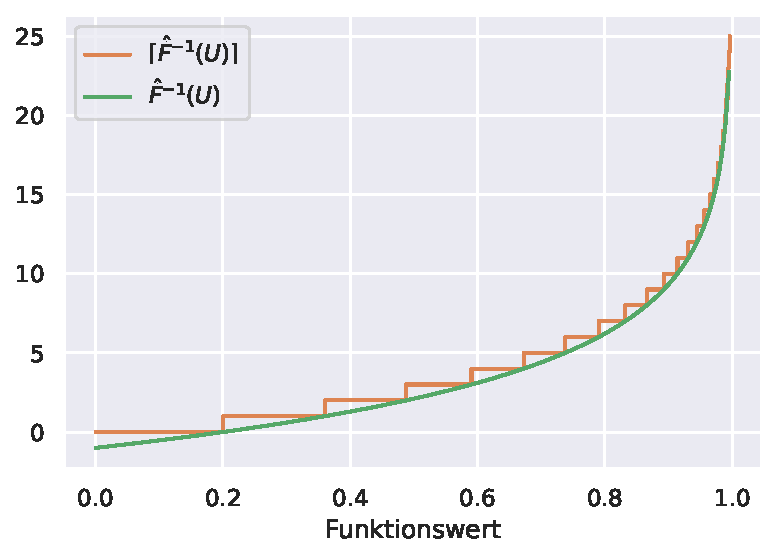
\includegraphics[width=0.5\textwidth]{data/geometric-distr-inv_hat.pdf}
    \end{center}
    \caption{Die in \cref{eq:inverse-hat} berechnet Umkehrfunktion $\hat F^{-1}(U)$}

\end{figure}

Zurück \aside{Inversionsmethode für geometrische Verteilung} zur geometrischen Verteilung mit $f(\ell) = (1-p)^\ell p$.
ObdA sei $0 < p < 1$ (da $X$ sonst eine Konstante ist).
Die kumulative Verteilungsfunktion lautet
\begin{equation}
    F(\ell)
    \ =\ p \sum_{i=0}^\ell (1-p)^\ell
    \ \stackrel{(*)}{=} \ p \frac{1 - (1-p)^{\ell+1}}{\underbrace{1 - (1-p)}_{=p}}
    \ = \ 1 - (1-p)^{\ell+1},
\end{equation}
wobei wir in $(*)$ die geschlossene Form der $\ell$-ten Partialsumme der geometrischen Reihe nutzen $\sum_{i=0}^\ell x^\ell = (1 - x^{\ell+1})/(1 - x)$.
Nun berechnen die Umkehrfunktion $\hat F^{-1}(U) = \ell$ indem wir $F(\ell) = U$ setzen und nach $U$ umformen.
Hierbei nehmen wir zunächst an, dass die Funktion stetig wäre (daher schreiben wir $\hat F ^{-1}$ statt $F^{-1}$):
\begin{eqnarray}
    U &=& F(\ell) = 1 - (1-p)^{\ell+1} \\
    \Leftrightarrow (1-p)^{\ell+1} &=& 1 - U \\
    \Leftrightarrow  (\ell+1) \log(1-p)  &=& \log(1 - U) \\
    \Leftrightarrow  \hat F^{-1}(U) := \log_{1-p}(1 - U) - 1 &=& \ell \label{eq:inverse-hat}
\end{eqnarray}

Schließlich erhalten wir $F^{-1}(U) = \lceil \hat F^{-1} (U) \rceil$ durch Aufrunden der gerade berechneten Funktion.
Zusammenfassen erzeugt \cref{alg:sample-geometric} eine geometrische Zufallsvariable $X$ mit Parameter $p$ in Zeit $\Oh{1}$:

\begin{algorithm}[H]
    \If{p=0}{Gebe $\infty$ zurück}
    \ElseIf{p=1}{Gebe $0$ zurück}
    \Else{$U \gets \text{ziehen uniform aus $[0, 1)$}$\;
    Gebe $\lceil \log_{1-p}(1 - U) - 1\rceil$ zurück.}
    \caption{Ziehen einer geometrischen Zufallsvariable}
    \label{alg:sample-geometric}
\end{algorithm}

\bigskip
\bigskip

\section{Effizientes Ziehen von \Gnm Graphen}\label{sec:sampling_gnm}
Trotz der strukturellen Ähnlichkeiten zwischen \Gnp und \Gnm Graphen unterscheiden sich ihre Generatoren signifikant.
Grund hierfür ist, dass während \Gnp \emph{in Erwartung} $n^2p$ Kanten erzeugen, müssen wir für \Gnm Generatoren sicherstellen, dass exakt $m$ zufällige Kanten produziert werden.

Ähnlich wie zuvor, reduzieren wir das Ziehen der richtigen Position von \emph{Einsen} in der Adjazenzmatrix auf den eindimensionalen Fall.
Im Folgenden werden wir also folgendes äquivalentes Problem lösen:
Ziehe uniform ohne Zurücklegen $k$ Elemente aus einer Menge $S = \set{s_1, \ldots, s_N}$ mit $|S| = N > k$.

\subsection{Reservoir Sampling}
Reservoir Sampling ist eine allgemeine Technik, die es uns erlaubt $k$ Elemente aus einem Datenstrom zu ziehen.
Hierbei müssen wir anfangs \emph{nicht} wissen, wie viele Elemente insgesamt im Strom sind.\footnote{
    Ein praktischer Anwendungsfall sind z.B. Iteratoren oder Generatoren, die in vielen Programmiersprachen genutzt werden.
    In Rust ist z.B. \texttt{rand::IteratorRandom::choose\_multiple} mittels Reservoir Sampling implementiert.
}
Im konkreten Fall besteht der Datenstrom also aus allen $s_i$ in beliebiger Reihenfolge.
Vereinfachend können wir also annehmen, dass der Strom mindestens $k$ Elemente enthält.

\begin{algorithm}[H]
    \KwIn{Eingabe: Datenstrom~$S$, Stichprobengröße~$k$}
    \KwOut{Array $R[1..k]$ mit $k$ zufällig ausgewählten Elementen}

    Initialisiere ein anfangs leeres Array $R$ mit Kapazität $k$\;

    \While{$|R| < k$}{
        $x \gets \text{nächstes Element aus $S$}$\;
        Füge $x$ an $R$ an\;
    }

    Setze $i = k$\;
    \While{$S$ nicht leer}{
        $x \gets \text{nächstes Element aus $S$}$\;
        $i \gets i + 1$\;
        $j \gets \text{ziehe uniform aus $[1, i]$}$\;
        \If{$j \le k$}{
            Ersetze $R[j] \gets x$\;
        }
    }

    Gebe $R$ zurück

    \caption{Reservoir Sampling}
    \label{algo:reservoir-sampling}
\end{algorithm}

\bigskip
\bigskip

\noindent
In \cref{thm:reservoir-sampling} zeigen wir die Korrektheit von \cref{algo:reservoir-sampling} für nur $k = 1$:
\begin{theorem}\label{thm:reservoir-sampling}
    Für $k=1$ liefert \cref{algo:reservoir-sampling} liefert ein uniform gewähltes Element $x\in S$.
\end{theorem}

\begin{proof}
    Sei $N$ die Länge des Stroms (ist dem Algorithmus nicht bekannt).
    Seien zudem $s_1, \ldots, s_N$ die Elemente in der Reihenfolge, in der sie aus dem Strom gelesen werden;
    oBdA gelte $s_i = s_j \ \Leftrightarrow\ i = j$ (d.h. alle Elemente sind unterschiedlich; falls nicht, können wir die Tupel $(s_i, i)$ betrachten).

    Sei $R$ die Zufallsvariable, welche die Ausgabe des Algorithmus modelliert.
    Dann ist zu zeigen, dass $\prob{R = s_i} = 1 / N$ für alle $1 \le i \le N$.
    \begin{eqnarray}
        \prob{R = s_i} &=& \prob{\text{$s_i$ wird in Runde~$i$ gewählt}} \cdot \prob{\text{$s_i$ wird nicht ersetzt}} \\
        &=& \frac{1}{i} \cdot \underbrace{\prod_{j=i+1}^N \frac{j-1}{j}}_{\text{Teleskop-Produkt}}
        = \frac{1}{i} \cdot \frac{i}{N} = \frac{1}{N}
    \end{eqnarray}

    \noindent Insbesondere gilt also, dass $\prob{R = s_i} = 1/N$ unabhängig von $i$ oder $s_i$ ist.
\end{proof}

\begin{exercise}
    Zeige die Korrektheit von \cref{algo:reservoir-sampling} indem du den Beweis von \cref{thm:reservoir-sampling} auf $k \ge 1$ verallgemeinerst.
    Dies lässt sich etwa über Induktion über die Datenstromlänge $|S|$ erreichen.
\end{exercise}

Wir können also \Gnm Graphen mittels Reservoir Sampling erzeugen.
Allerdings entspricht jede potentielle Kante einem Element in $S = V \times V$, für das wir je $\Theta(1)$ Arbeit verrichten müssen;
somit folgt eine Gesamtlaufzeit von $\Theta(n^2)$.

\subsection{Ziehen mit Lookups}
Im Folgenden skizzieren wir einen alternativen Ansatz um $k$~Elemente ohne Zurücklegen aus dem Universum~$S$ zu ziehen; dieser basiert auf \cite{batagelj2005efficient}.
Dieser nutzt das Grundgerüst in~\cref{algo:basis-ziehen-ohne-zuruecklegen}, das wir um einige Details erweitern müssen, um eine praktisch schnelle Implementierung zu erreichen:

\begin{algorithm}[H]
    \KwIn{Eingabe: Universum~$S$, Stichprobengröße~$k$}
    \KwOut{Menge $R$ mit $k$ zufällig ausgewählten Elementen}

    Initialisiere $R = \emptyset$\;

    \While{$|R| < k$}{
        $x \gets $ zufälliges Element aus $S$\;
        \If{$x \not\in R$}{
            $R \gets R \cup \set{x}$
        }
    }

    Gebe $R$ zurück

    \caption{Basisalgorithmus für Ziehen ohne Zurücklegen}
    \label{algo:basis-ziehen-ohne-zuruecklegen}
\end{algorithm}

\bigskip

Wir messen die Geschwindigkeit des Algorithmus zunächst nur indirekt, indem wir die Anzahl der Iterationen der \texttt{while}-Schleife zählen:

\begin{lemma}\label{lemma:basis-ziehen-ohne-zuruecklegen-versuche}
    \Cref{algo:basis-ziehen-ohne-zuruecklegen} verwendet in Erwartung $N \log(N/(N-k+1)) + \Oh{1}$ Versuche (Iterationen der \texttt{while}-Schleife) um aus $S$ mit $|S| = N$ exakt $1 \le k < N$ Elemente zu ziehen.
\end{lemma}

\begin{proof}
    Der Algorithmus baut $R$ inkrementell auf: wir beginnen mit $|R| = 0$ und fügen dann schrittweise je ein Element hinzu.
    Sei $X$ eine Zufallsvariable, die beschriebt, wie viele Iterationen der Algorithmus benötigt um $R$ zu erzeugen.
    Ferner seien $X_1, \ldots, X_k$ Zufallsvariablen, wobei $X_i$ beschriebt, wie viele Versuche benötigt werden um das $i$-te Elemente zu finden (d.h. um $R$ von $|R| = i - 1$ auf  $|R| = i$ zu heben).
    Per Konstruktion gilt $X = \sum_{i=1}^k X_i$ und aufgrund der Linearität des Erwartungswertes folgt

    \begin{equation}
        \expv{X} = \expv{\sum_{i=1}^k X_i} = \sum_{i=1}^k \expv{X_i}. \label{eq:basis-ziehen-ohne-zuruecklegen_expvX}
    \end{equation}

    Wir können also zunächst die Erwartungswerte $\expv{X_i}$ isoliert betrachten.
    Unmittelbar bevor wir das $i$-te Element ziehen, haben wir $i-1$ Elemente bereits bestimmt, d.h. $|R| = i - 1$.
    Mit Wahrscheinlichkeit $q_i = (i-1) / N$ erwischen wir also ein bereits gezogenes Element und versuchen es erneut.
    Mit Wahrscheinlichkeit $p_i = 1 - q_i = (N - (i - 1)) / N$ ziehen wir aber ein Element, dass noch nicht Teil von $R$ ist.
    Es gilt also

    \begin{align*}
        \prob{X_i = 1}            & = p_i                  \\
        \prob{X_i = 2}            & = (1 -p_i) p_i         \\
        \vdots         \quad\quad & = \quad\quad \vdots    \\
        \prob{X_i = 1 + \ell}     & = (1- p_i)^{\ell} p_i.
    \end{align*}

    Die Zufallsvariable $X_i - 1$ ist also geometrisch verteilt mit Erfolgswahrscheinlichkeit~$p_i$.
    Es gilt daher $\expv{X_i} = 1 / p_i = N / (N - i + 1)$. Durch Einsetzen in \cref{eq:basis-ziehen-ohne-zuruecklegen_expvX} erhalten wir:
    \begin{align}
        \expv{X} & = \sum_{i=1}^k \frac{N}{N-(i-1)} = \sum_{i=0}^{k-1} \frac{N}{N - i}                                      \\
                 & = N \sum_{i=N-k+1}^N \frac{1}{i}                                                                         \\
                 & = N \left[ \left( \sum_{i=1}^N \frac{1}{i} \right) - \left( \sum_{i=1}^{N-k} \frac{1}{i} \right) \right] \\
                 & = N \left[ H_N - H_{N-k} \right]
    \end{align}

    Im letzten Schritt nutzen wir die Definition $H_t = \sum_{i=1}^t 1/i$, also die $t$-te Partialsumme der Harmonischen Reihe.
    Es gilt, dass $H_t = \ln t + \gamma + 1/(2t) + \varepsilon_t$, wobei $\gamma \approx 0.5772$ die Euler–Mascheroni Konstante ist und $0 \le \varepsilon_t \le N^{-2}/8$ ein verschwindender Fehlerterm ist.
    Es folgt also:
    \begin{align}
        \expv{X} & = N \left[ H_N - H_{N-k} \right]                      \\
                 & \le N \left[ \ln N - \ln (N - k + 1) \right] + \Oh{1} \\
                 & = N \ln \frac{N}{N - k + 1} + \Oh{1}
    \end{align}
\end{proof}

\noindent
\begin{figure}
    \begin{center}
        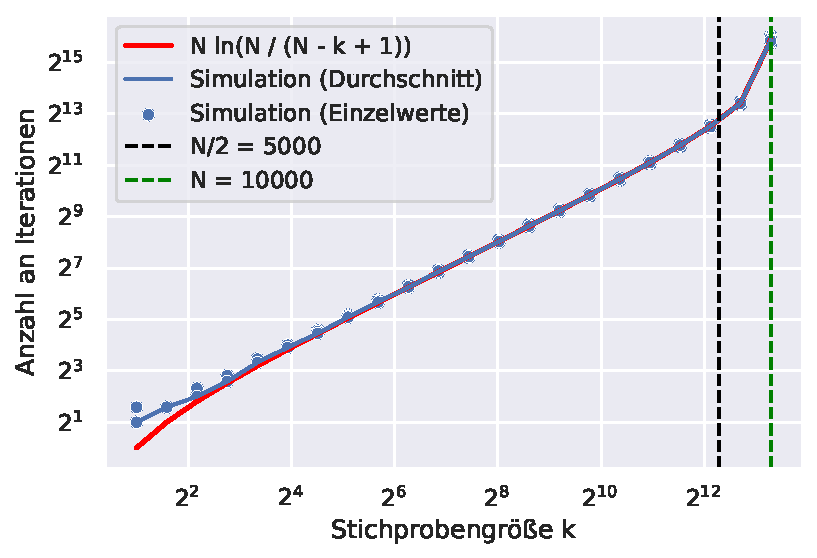
\includegraphics[width=0.5\textwidth]{data/gnm_iterationen.pdf}%
        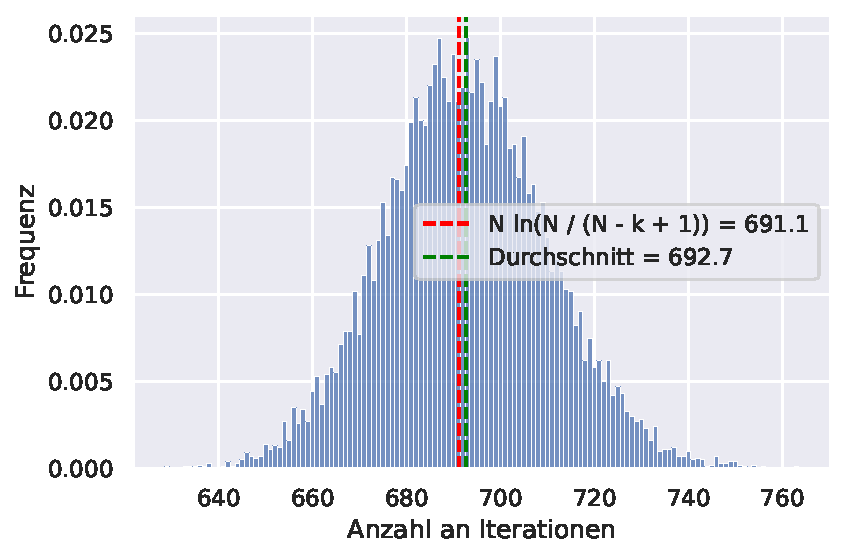
\includegraphics[width=0.5\textwidth]{data/gnm_iterationen_hist.pdf}
    \end{center}
    \caption{Simulation von \cref{algo:basis-ziehen-ohne-zuruecklegen} (ohne Komplementbildung).
        \textbf{Links}: $N=10\,000$ und $2 \le k \le 3N/4$; für jeden Parameter wurden 1\,000 unabhängige Simulationen ausgeführt.
        \textbf{Rechts}: $N=1\,000$, $k = N/2$. Es wurden 10\,000 unabhängige Simulationen ausgeführt.
    }
    \label{fig:ziehen-ohne-zuruecklegen-iterationen}
\end{figure}

Beobachte, dass die Analyse im Beweis von \cref{lemma:basis-ziehen-ohne-zuruecklegen-versuche} sehr eng ist.
Wie wir in \cref{fig:ziehen-ohne-zuruecklegen-iterationen} sehen, gilt für relativ kleine $N$ schon $\expv{X} \approx N \ln \frac{N}{N - k + 1}$.

\begin{exercise}
    Zeige, dass $N \ln \frac{N}{N - k + 1} = \Oh{k}$ für $k \le N / 2$.
\end{exercise}

\bigskip

\Cref{lemma:basis-ziehen-ohne-zuruecklegen-versuche} besagt, dass \cref{algo:basis-ziehen-ohne-zuruecklegen} für $k \le N / 2$ erwartet $\Oh{k}$ Iterationen ausführt und somit (in Erwartung) optimal ist.
Nur für $k \to N$ wird der $\log$-Faktor asymptotisch relevant, und wir bekommen eine suboptimale Laufzeit von $\Omega(N \log N)$.

Auf \aside{Komplementbildung stellt sicher: $k \ge N /2$} der einen Seite sollte das für \emph{übliche} Graphen kein Problem sein (sie sind dünn und daher $k \ll N$); dennoch lässt sich das Problem einfach vermeiden.
Für $k > N / 2$ können wir zunächst das Komplement~$\bar R$ mit  $| \bar R | = N - k < N/2$ ziehen und dann alle Elemente außer solche in $\bar R$ ausgeben.
Zwar benötigt die Komplementbildung $R = \bar{\bar R}$ während der Ausgabe $\Theta(N)$ Zeit, allerdings hat die Ausgabe ebenfalls Größe $\Omega(N)$, wodurch das asymptotisch optimal bleibt.

\subsection{Konzentration um den Erwartungswert}
Bisher haben wir uns darauf konzentriert Performance \emph{in Erwartung} zu analysieren.
In der Praxis kann das aber manchmal zu wenig sein:
wir stellen uns eine Implementierung vor, die in 99~\% der Fälle in 1\,s durchläuft aber in 1~\% der Ausführungen 101\,s benötigt.
Die durchschnittliche (\qq{erwartete}) Laufzeit wären also 2\,s.
Wenn wir unsere Pipelines darauf auslegen, kann das zu (im schlimmsten Fall kaskadierenden) Timeouts führen.

\Cref{fig:ziehen-ohne-zuruecklegen-iterationen} (rechts) scheint zu zeigen, dass \cref{algo:basis-ziehen-ohne-zuruecklegen} nicht in diese Kategorie fällt.
Unter 10\,000 Ausführung ist die größte Abweichungen vom Mittelwert nur rund 12\,\%.
Um Beobachtungen wie diese zu formalisieren, nutzt man häufig folgende Definition:

\begin{definition}
    Eine \aside{mit hoher Wahrscheinlichkeit} Eigenschaft~$X$ gilt \emph{mit hoher Wahrscheinlichkeit} (with high probability, whp),
    wenn für einen hinreichend großen Parameter $n$ die Gegenwahrscheinlichkeit $\prob{\lnot X} \le 1/n$ nicht übersteigt.
\end{definition}

In anderen Worten: je \qq{größer} unser Problem wird, desto unwahrscheinlicher sind extreme Ausreißer.
In der Regel ist der Parameter aus dem Kontext klar und wird daher in der Literatur oft nicht erwähnt (im folgenden Lemma wäre es $k$):

\begin{lemma}
    \Cref{algo:basis-ziehen-ohne-zuruecklegen} verwendet mit hoher Wahrscheinlichkeit \Oh{k} Iterationen für $k \le N/2$.
\end{lemma}

\begin{proof}
    Wir verwenden dieselbe Modellierung wie im Beweis von \cref{lemma:basis-ziehen-ohne-zuruecklegen-versuche}:
    Sei $X = \sum_{i=1}^k X_i$ die Gesamtanzahl an Iterationen und $X_i - 1$ geometrisch verteilt mit Erfolgswahrscheinlichkeit~$p_i$.

    Da $k \le N/2$, ziehen wir zu jedem Zeitpunkt mindestens mit Wahrscheinlichkeit $1/2$ ein neues Element, d.h. $p_i \ge 1/2$ für alle $i \ge 1$.
    Um die harmonische Reihe zu vermeiden, nutzen wir eine schlechtere Abschätzung, bei der wir alle $p_i = 1/2$ auf den minimalen Erfolgswert setzen.
    Sei $X' = \sum_{i=1}^k X'_i$ diese Verteilung und $X'_i - 1$ geometrisch mit Erfolgswahrscheinlichkeit $1/2$.

    \noindent
    Für einen beliebigen Grenzwert~$t$ gilt also
    \begin{equation}\label{eq:xprimet_groesser_xt}
        \prob{X > t} \le \prob{X' > t}.
    \end{equation}

    Wir können nun unsere Worst-Case Abschätzung $X'$ auch alternativ interpretieren:
    Wir werfen solange Münzen bis wir $k$ mal \qq{Kopf} gesehen haben.
    Die Anzahl der Versuche entspricht dann $X'$.

    Wir formalisieren diese alternative Idee:
    Sei $Y^{(t)} = \sum_{i=1}^t Y_i$ wobei $Y_i$ unabhängige Zufallsvariablen mit $\prob{Y_i = 1} = 1/2$ sind.
    Per Definition gilt
    \begin{equation}
        \prob{X > t}
        \quad \stackrel{\text{Eq. \ref{eq:xprimet_groesser_xt}}}{\le} \quad
        \prob{X' > t}
        \quad = \quad
        \prob{Y^{(t)} < k}
        \quad \le \quad
        \prob{Y^{(t)} \le k}
    \end{equation}

    \noindent
    Außerdem gilt $\expv{Y^{(t)}} = t/2$.
    Da $Y_i$ unabhängige Bernoullizufallsvariablen sind, hält die Chernoff-Ungleichung:
    \begin{align}
         &                                     & \prob{Y^{(t)} \le (1-\delta) \expv{Y_t}} & \le \exp\left(-\delta^2 \expv{Y^{(t)}} / 2\right)                  \\
         & \stackrel{\delta:=1/2}{\Rightarrow} & \prob{Y^{(t)} \le t / 4}                 & \le \exp\left(-(1/2)^2 (t/2) / 2\right) = \exp\left( -t/16 \right)
    \end{align}

    \noindent Im letzten Schritt wählten wir $\delta = 1/2$; nun setzen wir $t = 4k$:
    \begin{align}
         &             & \prob{Y^{(4k)} \le k} & \le \exp(-k/4) \le 1/k \quad \text{für } k \ge 9 \\
         & \Rightarrow & \prob{X > 4k}         & \le 1/k
    \end{align}

    \noindent
    Es folgt $\prob{X \le 4k} \ge 1 - 1/k$. Somit gilt $X < 4k$ mit hoher Wahrscheinlichkeit.
\end{proof}

Welche Datenstruktur benötigen wir für $R$? Sie sollte Existenzanfragen ($x \in R$?) und Einfügen ($R \gets R \cup \set{x}$) effizient durchführen können.
Ein Hashset unterstützt beide Operationen in erwartet konstanter Zeit, wodurch sich eine erwartete Laufzeit von $\Oh{k}$ ergibt; dies ist optimal in Erwartung.

Für praktische Implementierungen kann es sich jedoch auch lohnen, das Hashset durch ein Bitset (d.h. ein Array in dem jeder Eintrag genau ein Bit groß ist) zu ersetzen.
Auf dem Papier benötigt ein Bitset $\Theta(N)$ viele Bits und ist somit in der Initialisierung teuer.
In der Praxis benötigt aber jeder Eintrag in einem Hashset mindestens 64 Bit, sodass ein Bitset bereits für $N / k > 64$ weniger Platz benötigt (das trifft etwa auf 30\,\% der Netzwerke in \cref{fig:kantenanzahl} zu).
Zusätzlich sind Existenzanfragen und Einfügeoperationen extrem schnell, wodurch ein Bitset oft einen lohnenswerten Kompromiss zwischen mehr Speicher für schnellere Ausführung darstellen kann.

\begin{widefigure}
    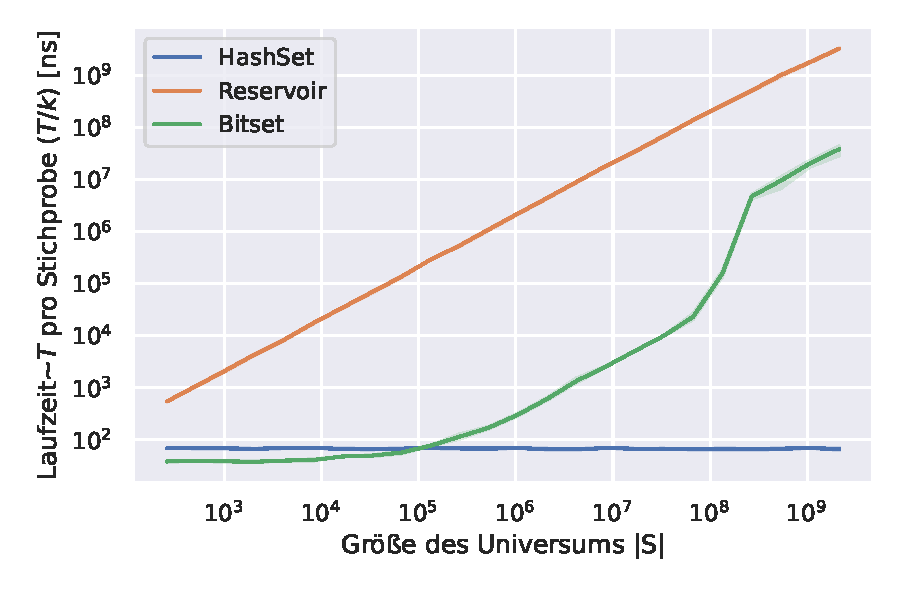
\includegraphics[width=0.32\textwidth]{data/gnm_scale0.pdf}\hfill
    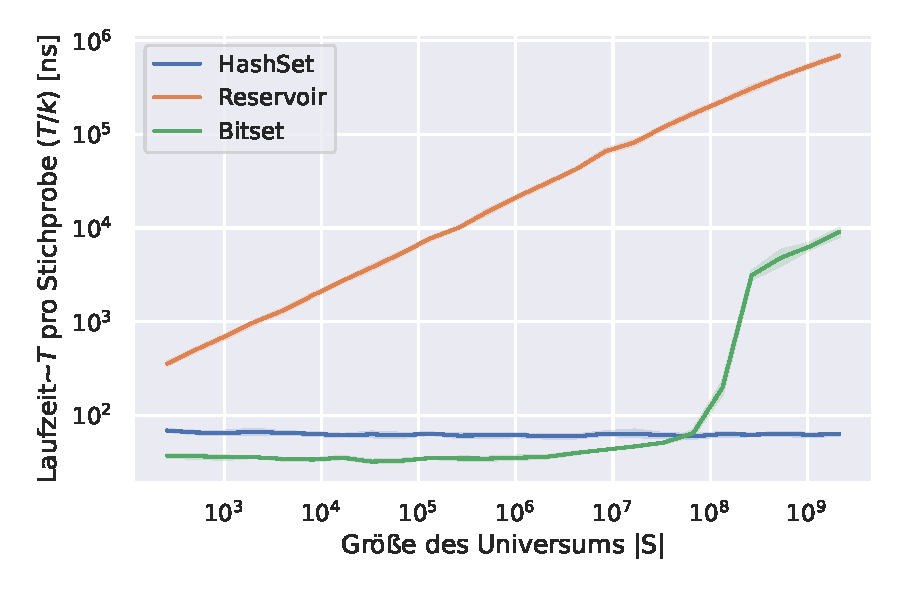
\includegraphics[width=0.32\textwidth]{data/gnm_scale1.pdf}\hfill
    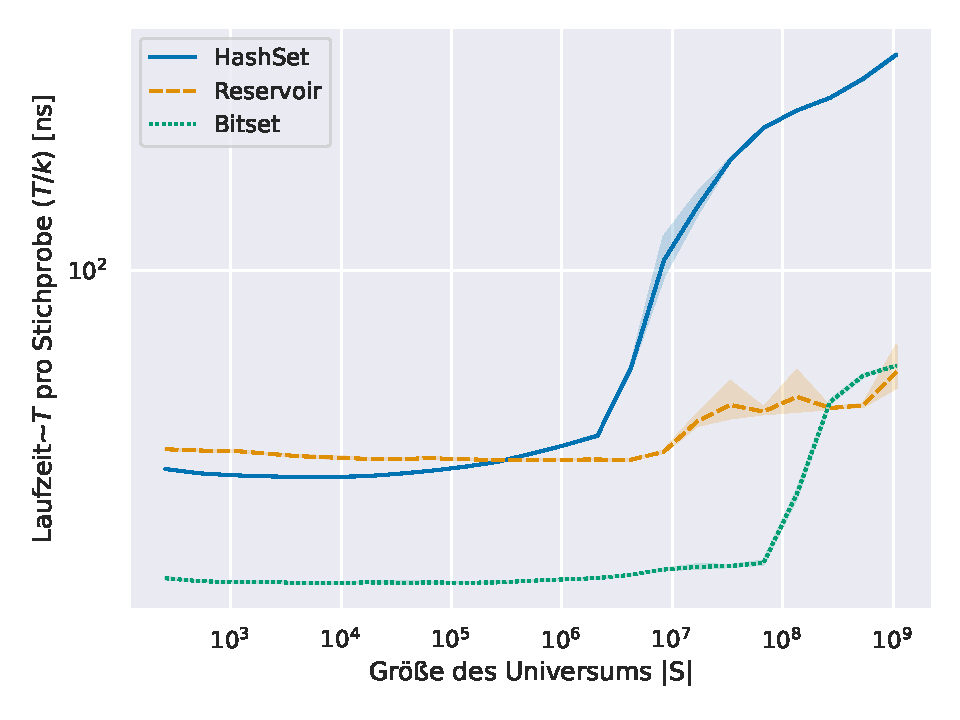
\includegraphics[width=0.32\textwidth]{data/gnm_scale2.pdf}

    \caption{
        Laufzeit~$T$ pro Sample~$k$ für das Ziehen von $k$ Elementen aus $S = \set{1, \ldots, N}$ als Funktion von $|S|$.\\
        \textbf{Links:} $k=10$, \textbf{Mitte: } $k = \sqrt{N}$, \textbf{Rechts: } $k = N / 4$.
    }
    \label{fig:benchmark_gnm_scale}
\end{widefigure}

In \cref{fig:benchmark_gnm_scale} stellen wir Laufzeitmessungen für folgendes Experiment dar.
Wir variieren die Größe unseres Universums $|S| = N$ von $2^8$ bis $2^{32}$ und betrachten drei Szenarien:
\begin{itemize}
    \item $k=10$: Trotz steigender Universumsgröße ziehen wir immer nur 10 Samples.
    \item $k=\sqrt{N}$: Die Stichprobengröße steigt langsam in der Universumsgröße (dieser Fall entspricht einem $\Gnm$ Graphen mit $m = \Theta(n)$).
    \item $k=N/4$: Jedes vierte Element des Universums wird ausgewählt.
\end{itemize}

\begin{exercise}
    Welche Effekte kannst du in \cref{fig:benchmark_gnm_scale} beobachten? Wie erklären sich diese?
\end{exercise}

Wir möchten uns aber nur auf einen zentralen Effekt in den Abbildungen konzentrieren, da dieser bei großen zufälligen Daten oft auftritt.\footnote{foreshadowing\ldots}
In \cref{fig:benchmark_gnm_scale} (rechts) beobachteten wir einen sprunghaften Anstieg der Zeit pro Element --- teils um fast einen Faktor 10.
Unsere Analysen sagen jedoch eine konstante Laufzeit pro gezogenem Element für $k = N/4$ voraus; einen sprunghaften Anstieg können sie nicht erklären.

Wir sind also im Algorithm-Engineering-Zyklus auf eine Diskrepanz zwischen Theorie und Praxis gestoßen!
Ist unsere Analyse falsch? Jaein.
In der Bestimmung der Laufzeit nutzen wir eine Unit-Cost Random-Access-Machine (d.h. wir gingen davon aus, dass jede Operation gleich viel Zeit benötigt).
Moderne Computer verfügen jedoch über ausgeklügelte Techniken, die gewisse Aspekte besonders beschleunigen.

Hierzu gehören die sog. Speicherhierarchien: Ein Prozessor kann nur auf Daten operieren, die sich auf dem physischen Chip befinden, genauer in den Registern.
Aus physikalischen und ökonomischen Gründen, gibt es aber nur sehr wenig \qq{Register-Speicher}.
Die meisten aktiven Daten werden daher im Arbeitsspeicher vorgehalten; dieser ist aber recht langsam.
Eine typische CPU kann in der Zeit, die es dauert ein Datum aus dem Arbeitsspeicher zu beziehen, etwa 100 bis 1000 Operationen ausführen.
Um dies aufzufangen, werden mehrere Caches eingefügt: die CPU \qq{rät} welche Daten in naher Zukunft benötigt werden und hält diese im schnelleren Cache vor.
Dies klappt aber mit Zufallsdaten oft nicht (sie sollen ja gerade \emph{nicht} vorhersehbar sein).

In \cref{fig:benchmark_gnm_scale} (rechts) sehen wir also genau den Punkt ab dem die Datenstrukturen nicht mehr in den Cache passen.
Für Hashset und Reservoir-Sampling nutzen diese Datenstrukturen etwa $64 k = 16 N$ Bits (das Hashset aufgrund des Load-Factors < 1 auch ein bisschen mehr).
Das Bitset benötigt $N$ Bits --- daher kommt hier der Performanceeinbruch auch später.

Um über diese qualitative Erklärung hinaus, das Verhalten analytisch zu erklären, benötigen wir also ein Maschinenmodell, das auch Speicherzugriffe berücksichtigt.
Dem widmen wir uns aber erst später.
Im Folgenden betrachten wir stattdessen eine Parallelisierung des Algorithmus --- dieselbe Strategie führt jedoch auch zu einem Generator, der zufällige Speicherzugriffe auf den Cache beschränken kann.
Wir brauchen zunächst ein Maschinenmodell für parallele Berechnungen.

\subsection{Fork-Join Parallelismus}
Das Fork-Join-Modell ist eine Erweiterung der Random-Access-Machine, welche die RAM um die zwei namesgebenenden Instruktionen erweitert.
Eine Berechnung startet als gewöhnliches sequentielles Programm, einem sog. Task.
Angenommen wir führen gerade $t_0$ aus, dann können wir die Berechnung in zwei \glqq Kindertasks\grqq{} $t_1$ und $t_2$ teilen \aside{fork} (\emph{forken}).
Beide Tasks werden unabhängig von einander ausgeführt, während $t_0$ ruht.
Sobald $t_1$ und $t_2$ fertig sind, kommt es zur Wiedervereinigung \aside{join} (\emph{join}):
$t_1$ und $t_2$ werden \glqq gelöscht \grqq, $t_0$ wieder geweckt und setzt seine Berechnung fort.
Betrachten wir das parallele Summieren $\sum_{i=1}^n x_n$ von Zahlen $X = (x_1, \ldots, x_n)$ als einfaches Beispiel:

\begin{algorithm}
    \SetKwProg{Fn}{Function}{}{end}
    \SetKwFunction{ParSum}{ParSum}
    \SetKwFunction{Fork}{Fork}
    \SetKwFunction{Join}{Join}
    \Fn{\ParSum{$X=(x_1, \ldots, x_n)$}}{
        \If{$n = 1$}{
            gebe $x_1$ zurück und beende Task\;
        }
        Berechne Mitte~$m \gets \lfloor n/2\rfloor$\;
        \Fork{$
                \underbrace{\ParSum{$X_L = (x_1, \ldots, x_m)$}}_{\text{Task $t_1$}}, \ \
                \underbrace{\ParSum{$X_R = (x_{m + 1}, \ldots, x_n)$}}_{\text{Task $t_2$}}
            $}\;
        $(s_1, s_2) \gets \Join{$t_1, t_2$}$\;
        gebe $s_1 + s_2$ zurück und beende Task
    }
    \caption{Parallele Summe im Fork-Join Modell}
    \label{algo:parallel_sum}
\end{algorithm}

In \cref{algo:parallel_sum} teilen wir die Eingabe rekursiv in zwei gleich große Teile (modulo Rundung) und berechnen die Teilsummen für beide rekursiv.
Sobald die Teilergebnisse vorliegen, summieren wir diese in $\Oh{1}$ Zeit und geben es als Gesamtergebnis zurück.
Dieses Schema funktioniert analog für alle assoziativen Operationen (z.B. Produkt, Min, Max).

In der Praxis findet man einige Software-Bibliotheken, die Fork-Join-Parallelismus zur Verfügung stellen;
für C++ etwa \texttt{Cilk} oder Intels \texttt{oneTBB}, für Rust \texttt{rayon}.
Diese praktischen Lösungen nutzen einen sog. Work-Stealing-Scheduler.

Grob \aside{Work Stealing} kann man annehmen, dass der Prozessor~$P_0$, der $t_0$ ausführte den Task $t_2$ als verfügbar bekannt gibt und dann selbst $t_1$ ausführt.
Wenn während der Ausführung von $t_1$ ein anderer Prozessor verfügbar ist, übernimmt dieser $t_2$.
In diesem Fall sind $t_1$ und $t_2$ also nebenläufig.
Wenn sich kein anderer Prozessor findet, wird $P_0$ den Task $t_2$ übernehmen, sobald $t_1$ beendet wurde.
Wir erhalten also ein dynamisches System, das (i) nicht wissen muss, wie viele Prozessoren es gibt, und (ii) auch relativ gut damit umgehen kann, dass $t_1$ und $t_2$ evtl. sehr unterschiedliche Laufzeiten haben.
Praktisch ist es kein Problem viel mehr Tasks zu erzeugen als es Prozessoren gibt.

Wir messen die Güte eines Fork-Join-Algorithmus mit zwei Eigenschaften:
\begin{enumerate}
    \item
          Die \aside{Arbeit / work} \emph{Arbeit} (engl. work) ist die Summe aller Instruktionen, die das Programm ausführt.
          Dies entspricht also der Laufzeit, wenn nur ein Prozessor zur Verfügung steht.
          Für \cref{algo:parallel_sum} ergibt sich die Arbeit als
          \begin{equation}
              W(n) = \begin{cases}
                  \Oh{1}                  & \text{falls } n = 1 \\
                  2 \cdot W(n/2) + \Oh{1} & \text{falls } n > 1
              \end{cases}
              = \Oh{n}.
          \end{equation}

          Der \aside{arbeits-optimal} Algorithmus leistet also asymptotisch nicht mehr Arbeit als die Laufzeit der besten sequentiellen Lösung; wir sagen er ist \emph{arbeits-optimal}.

    \item
          Der \aside{Span / Parallel Depth} Span (engl. span oder parallel depth) misst die Anzahl der Instruktionen auf einem kritischen Pfad (d.h. eine längste Folge abhängiger Schritte).
          Dies entspricht der Laufzeit, wenn wir unbeschränkt viele Prozessoren zur Verfügung haben.
          In \cref{algo:parallel_sum} müssen wir also analysieren, wie viele Instruktionen vor und nach dem Fork/Join Paar erforderlich sind und wie tief die Rekursion läuft:
          \begin{equation}
              S(n) = \underbrace{\Oh{1}}_\text{Arbeit vor/nach Fork/Join} + \underbrace{S(n/2)}_\text{Rekursion} = \Oh{\log n}.
          \end{equation}
\end{enumerate}

Wenn wir ausreichend Prozessoren zur Verfügung haben, können wir also $n$ Zahlen in Zeit $\Oh{\log n}$ summieren.
Zu ähnlichen Ergebnissen kommt man auch in anderen parallelen Maschinenmodellen (z.B. P-Rams).

\subsection{Rekursives Ziehen}
In \cref{algo:parallel_sum} haben wir bereits ein gutes Grundgerüst für parallele Algorithmen gesehen:
wenn wir es schaffen das Problem \emph{schnell} in unabhängige Hälften zu teilen und dann rekursiv zu bearbeiten, sind wir auf einem guten Weg.
Bezogen auf unser Problem, $k$~Stichproben aus $N$~Elementen zu ziehen, haben wir zwei Dimensionen:
\begin{enumerate}
    \item Teile $S$ deterministisch in $S_1$ und $S_2$: Wir können das Universum~$S$ mit $|S| = N$ in zwei Hälften $S_1$ und $S_2$ partitionieren mit $|S_1| = \lfloor N / 2 \rfloor$.
          Dann stellt sich die Frage: was ist die Anzahl~$k_1$ der Samples aus $S_1$, bzw. $k_2$ aus $S_2$. Klar ist nur $k_1 + k_2 = k$.

    \item Teile $k$ deterministisch in $k_1$ und $k_2$: Wir können die Stichproben teilen, d.h. $k_1 = \lfloor k/n \rfloor$ wählen; dann müssen wir jedoch eine unbekannte Partitionierung von $S$ finden.
\end{enumerate}

Auf den ersten Blick wirkt die zweite Variante zielführender.
Es ist vorteilhaft, wenn beide Teilprobleme etwa die gleiche Stichprobenanzahl haben, da die Arbeit in dieser Anzahl skalieren soll.
Tatsächlich liefert aber die erste Variante einfachere Algorithmen, die auch keine signifikanten Probleme mit unbalancierten Teilproblemen haben.

\begin{figure}[t]
    \begin{center}
        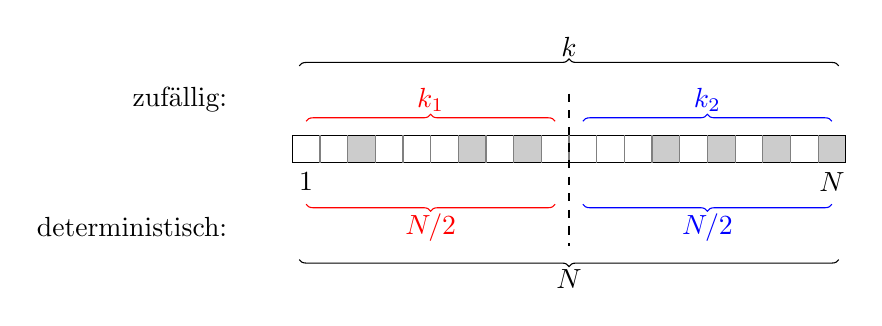
\begin{tikzpicture}
            \foreach \x in {-8, -4, -2, 3, 5, 7, 9} {
                    \node[inner sep=0, minimum size=1em, fill=black!20, anchor=west] at (\x em, 0) {};
                }

            \node[draw, minimum height=1em, minimum width=20em] at (0,0) {};
            \node[anchor=north] at (-9.5em, -0.5em) {1};
            \node[anchor=north] at ( 9.5em, -0.5em) {$N$};

            \foreach \x in {-9,...,9} {
                    \path[draw, black!50] (\x em, 0.5em) to ++(0, -1em);
                }

            \path[draw, thick, dashed] (0, 2em) to (0, -3.5em);

            \draw[decorate, decoration = {brace}] (-9.75em,3em) to node[above] {$k$} ++(19.5em,0);
            \draw[red,  decorate, decoration = {brace}] (-9.5em,1em) to node[above] {$k_1$} ++(9em,0);
            \draw[blue, decorate, decoration = {brace}] ( 0.5em,1em) to node[above] {$k_2$} ++(9em,0);

            \node[anchor=east] at (-12em, 1.8em) {zufällig:};

            \draw[decorate, decoration = {brace, mirror}] (-9.75em,-4em) to node[below] {$N$} ++(19.5em,0);
            \draw[red,  decorate, decoration = {brace, mirror}] (-9.5em,-2em) to node[below] {$N / 2$} ++(9em,0);
            \draw[blue, decorate, decoration = {brace, mirror}] ( 0.5em,-2em) to node[below] {$N / 2$} ++(9em,0);

            \node[anchor=east] at (-12em, -2.8em) {deterministisch:};

        \end{tikzpicture}
    \end{center}
    \caption{
        Ziehen von $k=7$ Stichproben aus $N=20$ Elementen ohne Zurücklegen; die grauen Elemente seien ausgewählt.
        Die linke Hälfte des Universums liefert $k_1$ Stichproben, die rechte $k_2$.
        Im gezeigten Beispiel gilt $k_1 = 3$ und $k_2 = 4$.
    }
    \label{fig:rekursive_k_aus_N}
\end{figure}


Wie in \cref{fig:rekursive_k_aus_N}, teilen wir also das Universum~$S$ in zwei gleich große Hälften $S_1$ und $S_2$.
Angenommen, wir täten dies nicht, wie viele Stichproben $k_1$ würde ein anderer Algorithmus aus $S_1$ ziehen?
Wir wissen es nicht genau, da $k_1$ eine Zufallsvariable ist --- sie ist Hypergeometrisch verteilt:
aus einer Gesamtpopulation von $N$ mit $k$~Treffern (d.h. die Elemente, die ein anderer Algorithmus gezogen hätte), ziehen wir $N_1$ Stichproben und erhalten $k_1$~Treffer.
In Erwartung sind es also $\expv{k_1} = k |S_1| / |S|$.

Analog zu den zufälligen Sprüngen in \cref{subsec:gnp_zufaellige_spruenge}, ziehen wir $k_1$ aus einer Hypergeometrisch Verteilung.
Dann setzen wir den Prozess bedingt auf $k_1$ fort:

\begin{algorithm}
    \SetKwProg{Fn}{Function}{}{end}
    \SetKwFunction{ParSelect}{ParSample}
    \SetKwFunction{Fork}{Fork}
    \SetKwFunction{Join}{Join}
    \Fn{\ParSelect{$S=(s_1, \ldots, s_N), k$}}{
        \If{$k = 1$}{
            $x \gets$ zufällig uniform aus $S$\;
            gebe $\set{x}$ zurück und beende Task\;
        }
        \BlankLine
        $N_L \gets \lfloor N / 2 \rfloor$\;
        $k_L \gets$ zufällig hypergeometrisch: ziehe $N_L$ Element aus $N$ mit $k$ Treffern\;
        \BlankLine
        \Fork{$
                \underbrace{\ParSelect{$S_L = (s_1, \ldots, s_{N_L}), k_L$}}_{\text{Task $t_1$}}, \ \
                \underbrace{\ParSelect{$S_R = (s_{N_L + 1}, \ldots, s_N), k - k_L$}}_{\text{Task $t_2$}}
            $}\;
        $(R_1, R_2) \gets \Join{$t_1, t_2$}$\;
        gebe $R_1 \cup R_2$ zurück und beende Task
    }
    \caption{Paralleles Ziehen von $k$ Stichproben aus $S$ ohne Zurücklegen}
    \label{algo:parallel_k_aus_N}
\end{algorithm}

\goodbreak

\noindent
Um die Performance von \cref{algo:parallel_k_aus_N} zu analysieren, treffen wir zwei Annahmen:
\begin{enumerate}
    \item Wir können $S$ in $\Oh{1}$ Zeit in zwei (fast) gleich große Hälften teilen.
          Das ist in vielen Fällen möglich:
          \begin{itemize}
              \item Für $\Gnm$ Graphen gehen wir davon aus, dass $S$ nur implizit existiert und das Intervall $[1, n^2]$ repräsentiert.
                    Dies können wir durch Verschieben der Intervallgrenzen trivial in $[1, n^2 / 2]$ und $[n^2/2 + 1, n^2]$ teilen.
              \item Wenn $S$ ein Array ist, können in die Rekursion Pointer auf den Anfang und das Ende des Teilproblems gegeben.
          \end{itemize}

    \item Die Operationen $R_1 \cup R_2$ läuft in konstanter Zeit.
          Das ist realistisch: da die Elemente in der Menge $S$ paarweise verschieden sind, wissen wir, dass $|R_1 \cup R_2| = |R_1| + |R_2| = k$.
          Es ist also kein Test auf Duplikate o.Ä. notwendig und es reicht aus $R_1$ und $R_2$ zu konkatenieren.
          Das ist mit verketten Listen (inkl. Endpointer) in $\Oh{1}$ Zeit möglich.
\end{enumerate}

\begin{exercise}
    Angenommen wir möchten $R$ als Array bekommen.
    Zeige, dass es möglich ist $R$ eingangs mit einer Kapazität von $k$ zu initialisieren, und dann in der Rekursion direkt in $R$ zu schreiben.
    Die Samples sollen dann in derselben relativen Reihenfolge wie in $S$ erscheinen.
\end{exercise}

\begin{lemma}
    \Cref{algo:parallel_k_aus_N} hat mit hoher Wahrscheinlichkeit einen Span von $\Oh{\log k}$ und benötigt in Erwartung $\Oh{k}$ Arbeit.
\end{lemma}

\begin{widefigure}
    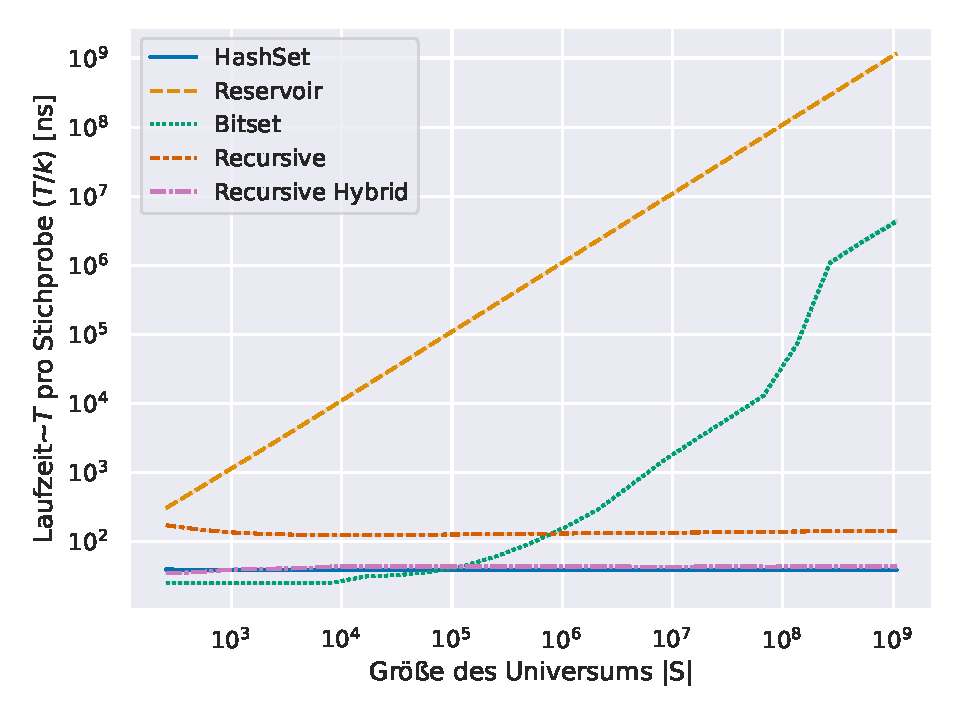
\includegraphics[width=0.32\textwidth]{data/gnm_recursive_scale0.pdf}\hfill
    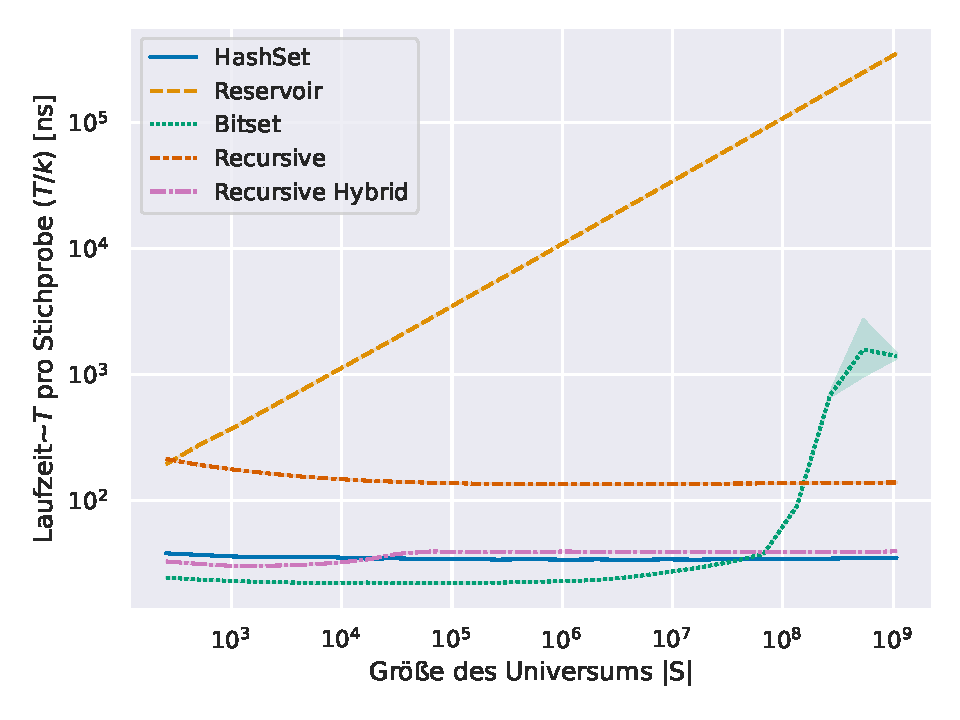
\includegraphics[width=0.32\textwidth]{data/gnm_recursive_scale1.pdf}\hfill
    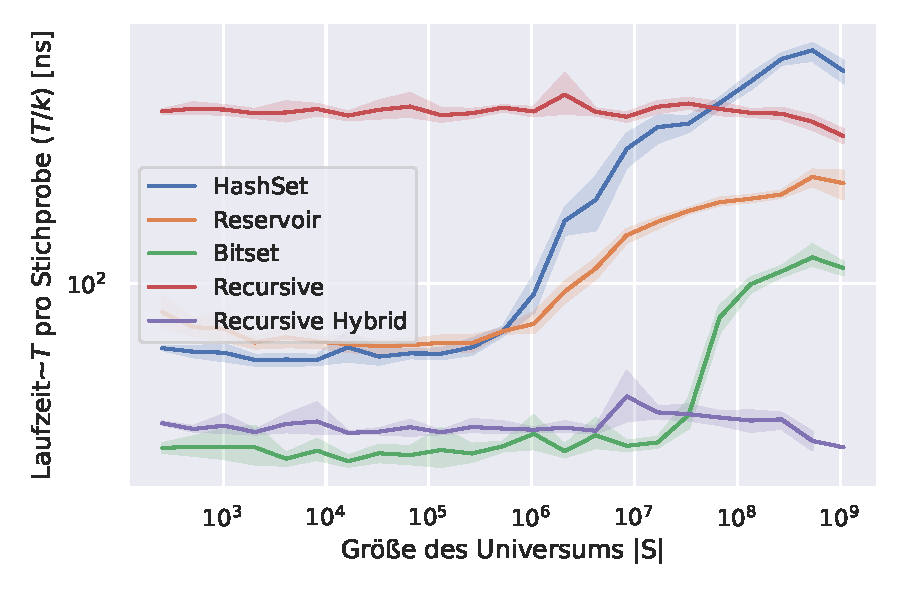
\includegraphics[width=0.32\textwidth]{data/gnm_recursive_scale2.pdf}

    \caption{
        Laufzeit~$T$ pro Sample~$k$ für das Ziehen von $k$ Elementen aus $S = \set{1, \ldots, N}$ als Funktion von $|S|$.\\
        \textbf{Links:} $k=10$, \textbf{Mitte: } $k = \sqrt{N}$, \textbf{Rechts: } $k = N / 4$.
    }
    \label{fig:benchmark_gnm_recursive_scale}
\end{widefigure}

Wir überspringen den Beweis; dieser lässt sich aber analog zu \cite{DBLP:journals/toms/Hubschle-Schneider22} führen.
Die Hauptideen sind: ein Span von $\Oh{\log N}$ folgt trivial wie in unserem Beispiel zum parallelen Summieren, dadurch dass wir in jedem Schritt die Größe von $|S|$ halbieren.
Um den Span jedoch auf $\Oh{\log k}$ zu reduzieren, müssen wir zeigen, dass sich auch die Stichprobengröße ungefähr gleich auf beide Teilprobleme verteilt.
Dies folgt aus der relativ kleinen Varianz der Hypergeometrischen Verteilung für hinreichend großes $k$.
Nur für sehr kleines $k$ laufen wir Gefahr, dass eines der beiden Teilprobleme alle Samples enthält;
das ist aber zum einen unkritisch (weil $|S|$ trotzdem halbiert wird und so die Dichte $k/N$ steigt) und zum anderen, wie wir gleich sehen werden, für praktische Implementierungen unerheblich.

Wie in \cref{fig:benchmark_gnm_recursive_scale} gezeigt, zeigt eine (sequentielle) Implementierung von \cref{algo:parallel_k_aus_N} ein gutes Skalierungsverhalten.
Die Laufzeit hängt nur von $\Oh{k}$ ab und steigt nicht für großes $N$ --- sie ist jedoch allgemein recht hoch (das Ziehen einer Hypergeometrischen Zufallsvariable ist recht langsam).
Dies \aside{Rekursionsstopper} ist ein sehr gängiges Problem in komplexen Algorithmen mit einer einfachen Lösung.
Wir verwenden den aufwendigeren Algorithmus nur so lange, wie es von Vorteil ist.
Wenn die Teilprobleme hinreichend klein sind und wir alle Prozessoren auslasten, schalten wir als \qq{Rekursionsstopper} auf spezielle Basisalgorithmen um, die sich besonders gut für kleine Teilprobleme eignen.
Der Hybridalgorithmus in \cref{fig:benchmark_gnm_recursive_scale} nutzt, für große $N$ den rekursiven Ansatz.
Für kleine Teilprobleme mit $N < 10\,000$ kommt  ---je nach Dichte $k/N$--- entweder BitSet oder HashSet zum Einsatz.

\section{Phasenübergänge in \Gnp und \Gnm}
Die ersten analytischen Ergebnisse von Zufallsgraphen betrafen das Verhalten von kombinatorischen Eigenschaften für verschiedene Dichten (d.h. $m/n$ bei $\Gnm$, bzw $p$ bei $\Gnp$) im Grenzwert für $n \to \infty$.
In \aside{Wir nutzen ungerichtete Graphen und setzen $N = \binom n 2$} diesem Kapitel werden wir uns auf ungerichtete Graphen konzentrieren.

Betrachten wir zunächst \Gnm Graphen.
Für diese zeigten Erd\H{o}s und R\'enyi bereits 1960 einige Schwellwerte an denen sog. Phasenübergänge stattfinden.
Für \emph{sehr} dünne Graphen mit $m(n) = o(\sqrt n)$, bewiesen sie etwa, dass diese wahrscheinlich nur isolierte Knoten und Kanten beinhalten.
Wir wollen uns an dieser Aussage ansehen, wie man die Wahrscheinlichkeit eines solchen Ereignisses abschätzen kann.

\begin{lemma}
    Sehr dünne $\Gnm$ Graphen mit $m = o(\sqrt n)$ haben für $n \to \infty$ wahrscheinlich keine Knoten mit mehr als einer Kante.
\end{lemma}

\begin{proof}
    Sei $p(n,m)$ die Wahrscheinlichkeit, dass keine zwei Kanten einen gemeinsamen Endpunkt haben.
    Wir vergleichen nun die Anzahl der möglichen Graphen mit der Anzahl der günstigen Graphen (d.h. ohne zwei Pfade).
    Zunächst beobachten wir, dass es $|\mathbb G(n,m)| = \binom N m = \binom{\binom n 2}{m}$ verschiedene $\Gnm$ Graphen gibt.
    Wie viele von diesen haben keine Knoten mit mindestens Kanten?

    Stellen wir uns dazu vor, dass wir die Kanten $E = \set{\set{u_1, v_1}, \ldots, \set{u_m, v_m}}$ erstellen, indem wir $2m$ Knoten $u_1, v_1, u_2, v_2, \ldots, u_m, v_m$ ziehen.
    Da keine zwei Kanten einen gemeinsamen Endpunkt haben sollen und Schleifen verboten sind, müssen wir also $2m$ \underline{verschiedene} Knoten ziehen!
    Es ist aber egal, in welcher Reihenfolge wir die $m$~Kanten ziehen und ob ein Endpunkt als $u_i$ oder $v_i$ gezogen wird.
    Die Anzahl ergibt sich also als
    \begin{align}
        \frac{
            \overbrace{\binom{n}{2m}}^\text{$2m$ verschiedene Knoten aus $n$}
            \overbrace{(2m)!}^\text{Mögliche Permutation von $2m$ Elementen}
        }{
            \underbrace{m!}_\text{Reihenfolge der Kanten egal\ \ \ }
            \underbrace{2^m}_\text{Reihenfolge in einer Kante egal}
        }.
    \end{align}

    \noindent
    Die wir jeden möglichen Graphen mit derselben Wahrscheinlichkeit ziehen, gilt
    \begin{align}
        \bar p(n, m) = \frac{\binom{n}{2m} (2m)!}{m! 2^m \binom{\binom n 2}{m}} \label{eq:wkeit_keine_zwei_kanten}
    \end{align}

    \noindent
    Wir werden im Folgenden eine \emph{untere} Schranke für $\bar p(n,m)$ zeigen.
    Dazu nutzen wir folgende Abschätzung von $\binom n k$

    \begin{align}
        \binom n k \approx \frac{n^k \exp\left(-\frac{k^2}{2n} - \frac{k^3}{6n^2}\right)}{k!}
        \quad\quad \text{für } k = o(n^{3/4}).
    \end{align}

    Der Einfachhalt halber verzichten wir auf die Analyse des Fehlers dieser Abschätzung.
    Es folgt
    \begin{align}
        p(n, m)
         & \ge \frac{\binom{n}{2m} (2m!)}{m! 2^m \binom{n^2/2}{m}}                                                                                   \\
         & = \frac{\textcolor{blue}{\binom{n}{2m}}(2m!)}{\textcolor{red}{\binom{n^2/2}{m}} m! 2^m}                                                   \\
         & \approx \frac{
        \textcolor{blue}{n^{2m} \exp\left(-2\frac{m^2}{n} - \frac{8m^3}{6n^2}\right)}\textcolor{red}{m!}(2m!)
        }{
        \textcolor{blue}{(2m)!}\textcolor{red}{\underbrace{(n^2/2)^m}_{=n^{2m} / 2^m} \exp\left(-2\frac{m^2}{n^4} - \frac{8m^3}{6n^6}\right)} m!2^m} \\
         & = \exp\left(-2\frac{m^2}{n} (1 - \frac{1}{n^3}) - \frac{8m^3}{6n^2} (1 - \frac{1}{n^4}) \right)                                           \\
         & \ge \exp\left(-2\frac{m^2}{n} - \frac{8m^3}{6n^2} \right)                                                                                 \\
         & \ge \exp\left(-4\frac{m^2}{n} \right) \quad \text{für hinreichend großes $n$}
    \end{align}

    Damit gilt also $\lim_{n \to \infty} p(n, m(n)) = 1$ falls $m(n) = o(n)$.
\end{proof}

Beobachte, dass \cref{eq:wkeit_keine_zwei_kanten} eine exakte Wahrscheinlichkeit ist, die wir erst im Nachgang von unten abschätzen.
Durch eine geeignete obere Schranke lässt sich zeigen, dass für $m \ge c \sqrt n$ für ein konstantes $c > 0$ (d.h. nicht von $n$ abhängig) die Wahrscheinlichkeit mindestens eines Knotens mit mindestens zwei Nachbarn gegen $1$ geht.
Wir sagen daher, dass \Gnm Graphen einen Phasenübergang mit Schwellwertfunktion $m(n) = \sqrt n$ haben.


\bigskip

Wir wechseln nun zu \Gnp Graphen.
Hier werden wir einen Beweis sehen, der die Unabhängigkeit aller Kanten ausnutzt.
Zuerst schauen wir uns aber einige wohlbekannte Phasenübergänge an.
Sei $\epsilon >0$ hinreichend klein.
Dann gilt:
\begin{itemize}
    \item Falls $np < 1 - \epsilon$ haben mit hoher Wahrscheinlichkeit alle Zusammenhangskomponenten Größe $\Oh{\log n}$.
    \item Falls $np = 1$ hat die größte Zusammenhangskomponente mit hoher Wahrscheinlichkeit Größe $\Theta(n^{2/3})$.
    \item Falls $np > 1$ gibt es mit hoher Wahrscheinlichkeit eine einzelne Zusammenhangskomponente mit Größe $\Theta(n)$.
          Keine andere Komponente hat mehr als $\Oh{\log n}$ Knoten.

    \item Falls $np < (1-\epsilon)\log n$ gibt es mit hoher Wahrscheinlichkeit einzelne Knoten ohne inzidente Kanten.
    \item Falls $np > (1+\epsilon)\log n$ ist der Graph mit hoher Wahrscheinlichkeit zusammenhängend.
\end{itemize}

\begin{exercise}
    Zeige ein möglichst großes $p(n)$ für das $\Gnp$ Graphen mit hoher Wahrscheinlichkeit keine Kanten haben.
\end{exercise}

Wir möchten nun das Verhalten um $np = 1$ besser verstehen und folgen einem algorithmischen Beweis von \cite{DBLP:journals/rsa/KrivelevichS13}.
Die Idee ist relativ einfach:
wir führen eine Tiefensuche auf einem $\Gnp$ Graphen aus, wobei die Nachbarschaft durch Ziehen von Einträgen in der Adjazenzmatrix erkundet wird.
Dann zeigen wir, dass für $np < 1$ so wenig Einsen vorhanden sind, dass es sehr unwahrscheinlich ist eine große Zusammenhangskomponente zu beobachten.
Für $np > 1$, hingegen, sehen wir ausreichend viele Einsen.

\subsection{Tiefensuche auf $\Gnp$}
Im Folgenden definieren wir eine klassische Tiefensuche (DFS) auf eine Weise, die für den folgenden Beweis hilfreich ist.
Implementieren sollte man sie so besser nicht...
Während einer DFS können wir die Knotenmenge~$V$ in drei Teilmengen $B$, $S$, $U$ partitionieren:
\begin{itemize}
    \item \underline Bearbeitete Knoten~$B$ sind Knoten, die besucht wurden und keine Kinder in $U$ mehr haben.
    \item Knoten in~$S$ werden gerade erkundet und liegen daher auf dem \underline Stack.
    \item \underline Unbekannte Knoten wurden noch nicht gefunden.
\end{itemize}

Bevor die DFS startet, gilt also $B = S = \emptyset$ und $U = V$.
Die Suche terminiert sobald $B = V$ und $S = U = \emptyset$.
Solange dies noch nicht der Fall ist, wird einer der folgenden Schritte ausführt:

\begin{enumerate}
    \item Falls $S \ne \emptyset$ sei $v$ der Knoten, der als letztes eingefügt wurde ($S$ ist ein Stack)
          \begin{enumerate}
              \item Falls $v$ einen Nachbarn $w \in U$ hat: entferne $w$ aus $U$ und füge $w$ in $S$ ein
              \item Falls nicht, ist $v$ vollständig bearbeitet: entferne $v$ aus $S$ und füge $v$ in $B$ ein
          \end{enumerate}
    \item Falls $S = \emptyset$ entnehme den ersten Knoten $v \in U$ und füge ihn in $S$ ein
\end{enumerate}

Um Uneindeutigkeiten zu vermeiden, fixieren wir die Knotenordnung.
Hierzu nehmen wir oBdA an, dass $V = \set{1, \ldots, n}$ natürliche Zahlen sind.
Die Mengen $V$ und $U$ seien aufsteigend geordnet, insbesondere werden immer die kleinsten passenden Elemente entnommen (in Schritten 1a und 2).
Weiter, sei $S$ ein Stack, d.h. das Element, das als letztes eingefügt wurde, wird als erstes entfernt.

Das Besondere an unser DFS ist, dass wir keine Kantenliste als Eingabe bekommen, sondern uns vorstellen, einen Strom von unabhängig zufälligen Bits $X_1, \ldots, X_N$ zu erhalten, wobei $\prob{X_i = 1} = p$.
Wenn wir nun in Schritt 1a einen Nachbar von $v$ suchen, iterieren wir gleichzeitig über $U$ und $X$.
Dann geben wir das erste $w$ zurück, dessen Bit gesetzt war (falls es existiert).
Wenn wir das nächste Mal mit Knoten $v$ zu Schritt 1a kommen, suchen wir nur nach $w' \in U$ mit $w' > w$ --- wir machen also an der Stelle weiter, an der wir einen Nachbarn gefunden haben.

\begin{exercise}
    Zeige, dass jeder Eintrag der Adjazenzmatrix höchstens einmal betrachtet wird und wir mittels der $X_i$ somit ein DFS auf \Gnp simulieren.
    Die zweite Beobachtung (s.u.) folgt hieraus.
\end{exercise}

\noindent
Wir werden später folgende Beobachtung ausnutzen:
\begin{itemize}
    \item In jeder Iteration wird ein Knoten entweder von $U$ nach $S$ (Schritt 1a oder 2) oder von $S$ nach $B$ (Schritt 1b) bewegt.
          Es gibt also einen stetigen Fortschritt und der Algorithmus terminiert nach $\Oh{n}$ Schritten.
    \item Zu jedem Zeitpunkt gilt, dass der Graph keine Kanten zwischen $U$ und $B$ hat; insb. ändern noch nicht entdeckte Kanten hieran nichts mehr.
    \item Alle Knoten in $S$ gehören zur selben Zusammenhangskomponente.
\end{itemize}

\subsection{Zusammenhangskomponenten für $np = (1-\epsilon)$ sind klein}
Wenn wir nun DFS ausführen, werden wir unsere Strukturaussagen zu \Gnp auf Eigenschaften Stroms von Zufallsbits reduzieren.
Die Hauptarbeit dieser Analyse leisten wir in \cref{lemma:dfs_kaum_einsen_in_X}.

Der \aside{union bound} Beweis des Lemmas nutzt eine übliche Struktur.
Wir möchten zeigen, dass etwas mit hoher Wahrscheinlichkeit nicht passiert, obwohl es viele Möglichkeiten $X_1, \ldots, X_n$ hierfür gibt.
Man schätzt also zunächst die Einzelwahrscheinlichkeiten~$\prob{X_i}$ ab (vereinfachend nimmt man oft an, dass die $X_i$ unabhängig sind).
Hier sollten sich extrem kleine Erfolgswahrscheinlichkeiten $\prob{X_i} \le 1/n^2$.
Dann schätzt man die Wahrscheinlichkeit, dass mindestens eins eintritt, einfach als Summe der Einzelwahrscheinlichkeiten nach oben ab.
Booles \aside{Booles Ungleichung} Ungleichung besagt:
\begin{align}
    \prob{\bigcup_{i=1}^n X_i} = \prob{\text{mindestens ein $X_i$ tritt ein}} \le \sum_{i=1}^n \prob{X_i}
\end{align}

\noindent
Nun können wir eine wichtige Eigenschaft unserer Zufallsbits zeigen.
Wir befinden uns zunächst im subkritischen Bereich, sprich unsere Analyse betrachtet Graphen mit $np \le (1 - \epsilon)$.

\begin{lemma}[basiert auf \cite{DBLP:journals/rsa/KrivelevichS13}]\label{lemma:dfs_kaum_einsen_in_X}
    Sei $\epsilon > 0$ \aside{kleines $\epsilon > 0$ \\ $N = \binom n 2$ \\ $p = (1 - \epsilon) / n$ \\ $k = (10 / \epsilon^2) \ln n$} eine hinreichend kleine Konstante und seien $X = (X_1, \ldots, X_N)$ unabhängige Zufallsvariablen, die Bernoulli mit Parameter~$p$ verteilt sind.
    %\begin{enumerate}
    %\item
    Sei $p = (1 - \epsilon) / n$ und $k = (10 / \epsilon^2) \ln n$.
    Dann gibt es mit hoher Wahrscheinlichkeit keine zusammenhängende Teilfolge (Intervall) mit Länge $nk$ (d.h. $X_i, \ldots, X_{i+nk}$) in dem mindestens $k$ Zufallsvariablen den Wert 1 haben.

    %\item Sei $p = (1 + \epsilon) /n$ und $N_0 = \epsilon n^2/2$.
    %      Dann gilt mit hoher Wahrscheinlichkeit $|\sum_{i=1}^{N_0} X_i - \epsilon(1+\epsilon)/2| \le n^{2/3}$.
    %      \qedhere
    %\end{enumerate}
\end{lemma}

\begin{proof}
    %Beginnen wir mit der ersten Aussage.
    Wir definieren $Y_i = \sum_{j=1}^{nk} X_{i+j-1}$ als die Anzahl an Einsen im Intervall, das mit $X_i$ beginnt.
    Aus Symmetrie können wir uns zunächst auf ein Intervall $Y_1$ beschränken.
    Mittels additiver Chernoff Ungleichung kann man zeigen
    \begin{align}
        \prob{Y_1 \ge k} < \exp\left(-\frac{\epsilon^2(1-\epsilon)}{3} \cdot \frac{10}{\epsilon^2} \ln n \right)
        = \exp\left(- \underbrace{(1-\epsilon)}_{\to 1} \frac{10}{3} \ln n \right)
    \end{align}

    Da die Behauptung nicht nur über ein Intervall~$Y_1$ spricht, sondern über alle $Y_1, \ldots, Y_{N-nk}$, benötigen wir noch einen \emph{union bound}.
    Hierfür betrachten wir die Einzelereignisse $Y_i \ge k$ für alle $i$:

    \begin{align}
        \prob{\exists i:\ Y_i \ge k} & \le \sum_{i=1}^{N-k} \prob{Y_i \ge k}                                                                                        \\                                                                      \\
                                     & \le N \cdot \prob{Y_1 \ge k}                                                                                                 \\
                                     & \le \frac{n^2}{2} \ \cdot\ \underbrace{\exp\left(- \underbrace{(1-\epsilon)}_{\to 1} \frac{10}{3} \ln n \right)}_{=o(1/n^3)}
                                     & \le \frac{1}{2n}
    \end{align}

    Da die Gegenwahrscheinlichkeit durch $1/2n$ nach oben beschränkt ist, gilt die Aussage mit hoher Wahrscheinlichkeit.
\end{proof}

Wir wissen also, dass für $p \le (1 - \epsilon) / n$, wir in $nk$ Zufallsbits ziemlich sicher keine $k$ Einsen finden.
Die Intuition für \Gnp ist also, dass wir in $k$ Zeilen der Adjazenzmatrix keine $k$ Nachbarn finden.
Diese $k$ Zeilen können also nicht zusammenhängend sein!
Wir formalisieren dieses Bauchgefühl in folgendem Theorem:

\begin{theorem}[basiert auf \cite{DBLP:journals/rsa/KrivelevichS13}]
    Sei \aside{$\Gnp$ mit $np = (1-\epsilon)$ hat nur Zusammenhangskomponenten mit $\Oh{\log n}$ Knoten.} $\epsilon > 0$ hinreichend klein.
    Ferner sei $G \sim \Gnp$ ein zufälliger Graph mit $np = (1 - \epsilon)$.
    Dann haben alle Zusammenhangskomponenten mit hoher Wahrscheinlichkeit eine Größe von höchstens $10 \epsilon^{-2} \ln n$.
\end{theorem}

\begin{proof}
    Beweis durch \qq{Widerspruch} (tatsächlich kein echter Widerspruch, da die Aussage ja nur mit hoher Wahrscheinlichkeit gelten soll).
    Nehmen wir an, es gibt eine Zusammenhangskomponente~$K$ mit mehr als $k = 10 \epsilon^{-2} \ln n$ Knoten.
    Betrachten wir die Phasen in der DFS während $K$ exploriert wird.

    Konkret betrachten wir den Moment, zu dem der $k+1$ Knoten entdeckt wird (dieser wird also gleich von $U$ nach $S$ bewegt).
    Seien $\Delta K = K \cap B$ die Knoten der Zusammenhangskomponente~$K$, die bereits fertig bearbeitet wurden.
    Dann gilt $|\Delta K \cup S| = |\Delta K| + |S| = k$; sonst hätten wir nicht eben den $k+1$ Knoten entdecken können.

    Den ersten dieser $k$ Knoten bekamen wir \qq{kostenlos}, da er in Schritt 2 von $U$ nach $S$ bewegt wurde, um die Suche in der neuen Zusammenhangskomponente zu starten.
    Jeder weitere Knoten musste über eine Kanten zu einem Knoten in $\Delta K \cup S$ entdeckt wurden sein.
    Da Kanten zu einer Eins in unseren Zufallsbits korrespondiert, müssen wir als beim Entdecken des $k+1$ Knoten genau $k$ Einsen gesehen haben.

    Von jedem Knoten in $\Delta K \cup S$ suchten wir nach höchstens $n$ Nachbarn (grobe Überabschätzung!).
    In anderen Worten: wir haben höchstens $k n$ Bits gelesen und dabei $k$ Einsen gefunden.
    Das passiert gemäß \cref{lemma:dfs_kaum_einsen_in_X} mit hoher Wahrscheinlichkeit nicht.
    Der \qq{Widerspruch} zur Annahme folgt.
\end{proof}

Durch geeignete Abschätzung, dass es für $np = (1 + \epsilon)$ \qq{viele} Einsen gibt, lassen sich folgende Resultate zeigen.
Mit hoher Wahrscheinlichkeit enthält $G \sim \Gnp$ \ldots
\begin{itemize}
    \item \ldots einen Pfad mit mindestens $\epsilon^2 n / 5$ Knoten.
    \item \ldots einen Kreis mit $\Theta(\epsilon^2) n$ Knoten.
    \item \ldots eine Zusammenhangskomponente mit mindestens $\epsilon n / 2$ Knoten.
\end{itemize}

Beobachte, dass die giant component deutlich größer ist als die Pfadlänge.
Dies ist inhaltlich richtig (und erwartet --- warum??), bedarf aber auch eine deutlich genaueren Abschätzung unserer Zufallsbits.

Weiter ist die $\epsilon^2$ Abhängigkeit der ersten beide Aussagen optimal.
Tatsächlich ist das Resultat zur Pfadlänge der Grund, weshalb wir uns eine Tiefensuche statt einer Breitensuche angesehen haben.
Wenn wir in der Tiefensuche jemals eine Stackgröße von $|S| = k$ erreichen, wissen wir, dass der untersuchte Graph einen Pfad mit mindestens $k$ Knoten enthält;
das gilt nicht für die Breitensuche!
Der Beweis zeigt also, dass wir ausreichend viele Einsen sehen, um ein hinreichend großen Stack zu bekommen.

\subsection{Existenz von großen Kreisen}
Zuletzt wollen wir uns noch eine Beweistechnik ansehen, bei der wir zwei geeignet parametrisiert $\Gnp$ durch Vereinigung ihrer Kantenmengen \qq{aufaddieren}.
Mit dieser Technik lässt sich aus der (mit hoher Wahrscheinlichkeit) Existenz eines Pfads mit $\alpha n$ Knoten $\alpha > 0$, die (mit hoher Wahrscheinlichkeit) Existenz eines Kreises mit $\Theta(\alpha n)$ Knoten folgern.
Hierzu ziehen wir einen weiteren $\mathcal G(n, p')$ Graphen mit ausreichend großen $p' = o(1/n)$.
Diese neuen Kanten fügen wir zu unserem ursprünglichen Graphen $G$ hinzu und erhalten $G' \sim \mathcal G(n, p'')$ mit $p'' \lessapprox p + p'$.
Da $p' = o(1/n)$ ist $p + p' = (1+\epsilon)/n + o(1/n)$ für $n \to \infty$ weiterhin durch $p$ dominiert.

Zur einfacheren Illustration nehmen wir $p' = n^{-3/2} = o(1/n)$ an.
Weiter betrachten wir die ersten und letzten $\ell = 2 n^x$ Knoten des Pfades mit hinreichend großem $x < 1$.
Es bleibt ein Mittelteil von $M$ Knoten \qq{übrig}:
\begin{align}
    M = \alpha n - 2\ell =\alpha n - 4 n^x =  n(\alpha - \underbrace{4n^{x - 1}}_{=o(1)\text{, da } x < 1})
\end{align}

Im Grenzwert von $n\to\infty$, sind also Präfix und Suffix des Pfades relativ zum Mittelteil $2\ell / M = o(1)$ asymptotisch verschwindet klein.

Es gibt aber $\binom{\ell}{2} \ge n^{2x}$ mögliche Kanten zwischen dem Präfix und dem Suffix.
Aus $G'$ bekommen wir also erwartet mehr als $n^{2x} p'$ Kanten --- eine reicht um einen Kreis, der länger als $M$ ist, zu schließen.
In unserem Beispiel mit $p = n^{-3/2}$ gilt:
\begin{align}
    n^{2x} p' = n^{2x - 3/2}
\end{align}

Wenn wir also $x = 3/4$ wählen, erwarten wir mindestens eine Kante, die dann den versprochenen Kreis schließt.
Für $x > 3/4$ existiert eine solche Kante mit hoher Wahrscheinlichkeit.

\subsection{Cliquen in \Gnp}
Gemäß der Definition einer Zusammenhangskomponente~$K \subset V$ in einem Graphen $G=(V,E)$ finden wir für jedes Knotenpaar $u, v \in K$ einen Pfad von $u$ nach $v$.
Cliquen~$C \subseteq V$ sind ein Extremfall dieses Konzeptes, da zwischen alle Konstituenten $u \ne v \in C$ eine direkte Kante existiert.
Nach unserer bisherigen Diskussion scheint es eine natürliche Frage zu sein, wie viele Knoten eine größte Clique in einem Graphen $G \sim \Gnp$ hat.

Zunächst analysieren wir, wie viele Cliquen der Größe $k$ wir erwarten können.
Beachte, dass $C$ genau dann eine Clique ist, wenn der durch $C \subset V$ induzierter Teilgraph genau $\binom{k}{2}$ Kanten mit $k = |C|$ hat.
Insbesondere darf der Teilgraph keine \emph{Nichtkanten} enthalten.
Da jede Kante existieren muss, ist es besonders einfach die Wahrscheinlichkeit $\prob{\text{$C$ ist Clique}}$ zu beschreiben:
\begin{align}
    \prob{\text{$C$ ist Clique}} = p^{\binom{|C|}{2}}
\end{align}

Wir müssen nur noch die Anzahl möglicher Cliquen finden.
Es gibt genau $\binom{|V|}{k}$ verschiedene Knotenteilmengen der Größe~$k$.
Analog zum Beweis von \cref{lemma:erwartete_kanten_in_gnp} können wir für jede eine Indikatorvariable~$I_C$ annehmen, wobei $\prob{I_C = 1} = \expv{I_C} = p^{\binom{|C|}{2}}$.
Durch die Linearität des Erwartungswertes folgt dann die erwartete Anzahl an Cliquen der Größe~$k$ als
\begin{align}
    \binom{|V|}{k} p^{k(k-1)/2}.
\end{align}

Wenn wir uns den Spezialfall von $\Gn$ (d.h. $\Gnp$ mit $p = 1/2$) ansehen, lässt sich zeigen, dass es eine Funktion $f(n) \approx 2\ln n$ gibt,
sodass eine größte Clique in $G \sim \Gn$ mit hoher Wahrscheinlichkeit entweder $f(n)$ oder $f(n)+1$ Knoten hat.
Diese können wir aufgrund der kleinen Größe relativ einfach finden!
Wenn wir alle möglichen Cliquen explizit enumerieren und prüfen, ergibt sich \qq{nur} eine quasipolynomielle Laufzeit von $2^{\Theta(\log^2 n)}$.
Der Zufall vermeidet also pathologische Strukturen und vereinfacht das eigentlich $\mathcal{NP}$-schwere Clique-Problem auf $\Gn$ (und auf $\Gnp$ mit $p \le 1/2$) deutlich.
